% Chapter Electrodes

\chapter{Electrodes Design with Electrostatic Simulation} % Main chapter title

\label{ChapterElectrodes} % Change X to a consecutive number; for referencing this chapter elsewhere, use \ref{ChapterX}

%----------------------------------------------------------------------------------------
%	BEGING CHAPTER
%----------------------------------------------------------------------------------------

Let me tell you about my work with an electrostatic simulation software called COMSOL.
That was quite nice. Just designing the detector and the aluminium electrodes with a beautiful and efficient interface.
Thanks to that, I could simulate a lot of configuration and geometry to probe for the finest results out there.
Finest meaning a lot of fiducial volume, good charge collection, and low electric capacity.
A usual impossible to solve problem which lead to a lot of trade-off in itself, without adding the issues about the heat channel.
But hey, I could obtain some nice plots and tables, check them out.


\section{Electrodes as Sensors for the Ionization Channel}

\subsection{Basics of the Ionization channel}
\label{par:basic-ion-channel}

The ionization channels aims at converting the ionization of the germanium into a voltage signal.
This is done with the use of aluminium electrodes acting as the terminals of a capacitor of capacitance $C$. When collecting an electric charge $\Delta Q$, a voltage $\Delta U$ is created across the capacitor such as:

\begin{equation}
C = Q \times U \quad \Leftrightarrow \quad U \times = \frac{C}{Q}
\label{eq:capacitor-basic}
\end{equation}

A high sensitivity of the ionization channel means that the created voltage $\Delta V$ is maximized. The equation \label{eq:capacitor-basic} shows that a low capacitance $C$ of the electrodes and a high collection of electric charge $\Delta Q$ increase the ionization channel response. While the amount of electric charge $\Delta Q$ can depend of the electric field shape, in the case of a theoretically perfect charge collection, the number of electron-hole pairs created and collected only depends on the recoil energy $E_R$ of the interacting particle $i$ and the associated quenching factor $Q^i(E_R)$ which is plotted in the figure \ref{fig:quenching-germanium}. This factor depends only on the material used as absorber, in our case Germanium.
The capacitance depends on the design of the detector, and is the one of the main quantities used to quantify the performance of a detector design.

\begin{figure}
\centering
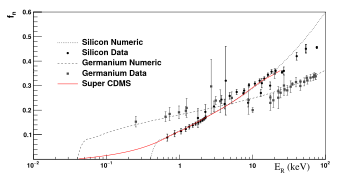
\includegraphics[width=0.48\textwidth]{Figures/Electrodes/quenching_germanium.png}
\caption{Quenching factor in the Germanium and Silicon as a function of the recoil energy $E_R$.}
\label{fig:quenching-germanium}
\end{figure}

\subsection{Reference detector designs}

The reference detector designs are used to illustrate the different concepts of the ionization channel. They are the result of the optimization of the ionization channel (presented later in this chapter) and thus presents very good performances. There are two reference design based on a 38g Germanium crystal of height 10mm and diameter 30mm: 

\begin{itemize}
	\item \textbf{Planar38}, with two collecting electrodes fully covering the planar faces and a part of the lateral face.
	\item \textbf{FID38}, with four interleaved circular electrodes (see the Fully InterDigitized design of EDELWEISS, if explained earlier). 
\end{itemize}


\begin{figure}
\centering
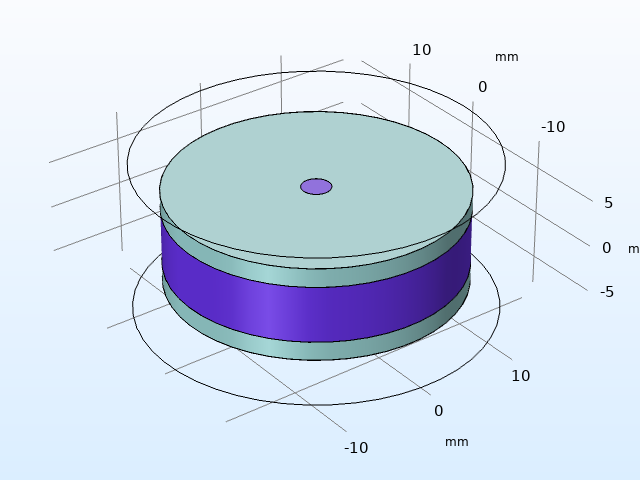
\includegraphics[width=0.48\textwidth]{Figures/Electrodes/planar38_3d.png}
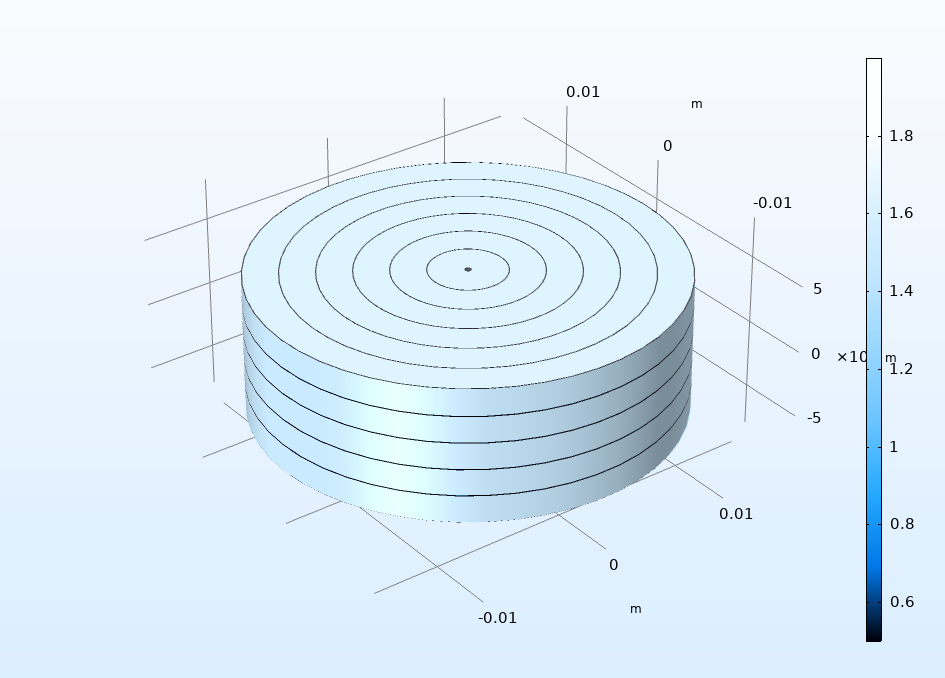
\includegraphics[width=0.48\textwidth]{Figures/Electrodes/fid38_3d.png}
\caption{
\textbf{Left:} Simulated geometry of the Planar38 detector. Electrodes are in grey, bare germanium crystal is colored purple.
\textbf{Right:} Simulated geometry of the FID38 detector. Electrodes are in black while the bare germanium crystal is colored cyan.
}
\label{fig:reference-design-3d}
\end{figure}

\subsection{Germanium as Semiconductor}

The material used as absorber for the detectors is semi-conducting High Purity Germanium [ref?].
This paragraph focuses on its characteristics and also compares it to materials used by others experiments using bolometers.

The use of semi-conducting Germanium as an absorber was first proposed by Taverdale? and Evvan [80, Emeline].
Along with an increase in temperature, a semi-conducting germanium also features a phenomenon of ionization caused by a particle interaction. Such electronic and nuclear recoils form electron-hole pairs of average energy $\epsilon = 3 eV/pair$. This energy corresponds to the gap energy separating the valence and conduction electronic bands in the germanium in its semi-conducting state accessible for temperature below 77K.

In order to understand the physical properties of a semi-conductor, we can consider the theory of energy bands. In a solid material, at rest electrons are occupying the lowest state of energy according to their fermion nature. This lowest state of energy are strongly linked to the nucleus, forming the valence electronic band of energy. Higher energy states are able to interact with neighboring atoms and compose the conduction electronic band of energy.global
conducting, not conducting, semi-conductor. Small gap. blablabla

The semi-conducting properties of a germanium crystal heavily depends on the impurities affecting it. With the Germanium element being of valence 4, there exist two kind of impurities:
\begin{itemize}
	\item acceptor impurities of valence 3 producing a p-type germanium,
	\item donor impurities of valence 5 producing an n-type germanium.
\end{itemize}
These impurities creates intermediary energy steps in the semi-conducting germanium band gap accessible to electric charges (as seen in figure \ref{fig:conduction-bands}). The presence if this intermediate accessible energy bands has several consequences on the ionization channel. It reduces the energy necessary to create an electron-hole pair, thus creating additional noise and biasing for the ionization channel. Then, it creates a trapping phenomenon which prevent electric charge carriers from reaching the electrodes. With trapped charges in the crystal, a counter electric field slowly generates, reducing the sensitivity of the electrodes. Finally, these impurities lower the global resistivity of the germanium crystal and increase the leakage current.
The semi-conducting germanium use as absorber thus should contain the lowest amount of impurities in order to have a detector with good performances.
The study of the trapping in EDELWEISS detector and the impact of impurities is presenting in [ref quentin 80].
We define $N_a$ and $N_d$ as the number of acceptor and donor impurities respectively. We  can have access (how?) to the absolute difference of this quantities $|N_a - N_d|$ which determine the number of available charge carriers.
The material used as absorber is High-Purity Germanium (HPGe) with an estimated:
$$ 10^{9} < |N_a - N_d| < 10^{10} \textsf{cm}^{-3}$$
which corresponds to less than one impurity atom for $10^{12}$ germanium atoms. With this material, low leakage currents of few pA can be achieved for the usual operating  electric field range of a few V/cm.

Ok, so here might be some mumbo jumbo concerning the p-n junction in a semi-conductor. Is it useful ? idk.
A recurring term is "depletion depth" which apparently is inversely proportional to the impurity concentration.
A germanium crystal with good performance should present a high resistivity obtainable with a high depletion depth.
As a result, the EDELWEISS and RICOCHET experiment use high purity germanium (HPGe) with special treatment [ref?] leading to a low impurity concentration of less than $10^{10}$ atoms.cm${-3}$ (1 impurity for $10^{12}$ germanium atoms) whereas a normal germanium crystal possesses a concentration of about $10^{13}$ atoms.cm${-3}$.

Comparing the germanium to silicium:
\begin{itemize}
	\item higher Z, so better quenching factor [lindhard]
	\item denser material, better for exposure
	\item low impurities, big depletion region
	\item low ionization energy (gap?)
	\item high conductivity (?)
\end{itemize}

\begin{figure}
\centering
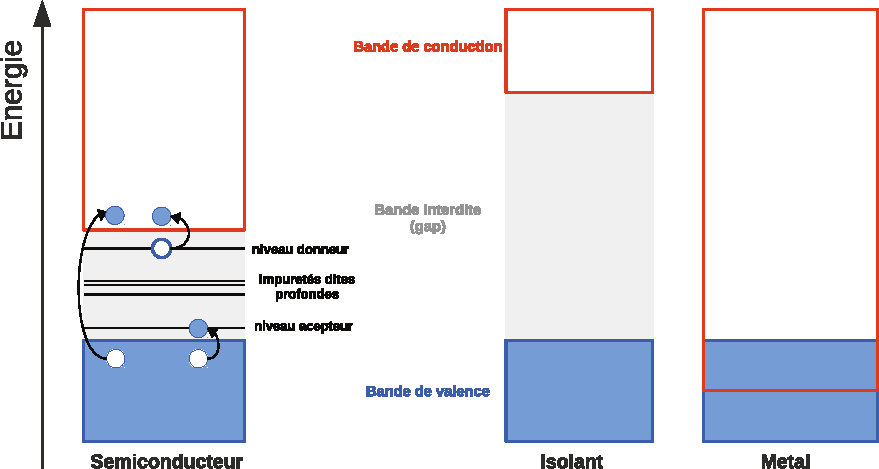
\includegraphics[width=\linewidth]{Figures/Electrodes/conduction_bands.pdf}
\caption{Scheme of the conduction bands for semiconductor, insulator and conductor materials.}
\label{fig:conduction-bands}
\end{figure}


\subsection{Electric Charge Drifting in Crystal}
\label{par:charge-drifting}
%{\color{red} Alex B. biblio here. Also explainin trapping, charge collection.}

The study of charge migration in EDELWEISS germanium crystal is presentend in [ref Emeline 82] taking into account the crystallographic structure of the germanium crystal. In this study, Alex.B simulates numerically the drifting of eletrons and holes in a 200g FID Edelweiss detector with bulk interaction of gamma-rays of energy 348keV. The charge trajectories are presented in the figure \ref{fig:charge-drifting}. He also follows the generation of the voltage signal on the electrodes. This is consistent with Ramo field theory which will be described later.

When interacting with the atoms of a germanium crystal, a particle deposits a so-called recoil energy. The word "recoil" references to the elastic diffusion of the incoming particle on a germanium nuclei, this is a nuclear recoil, or the elastic diffusion of the electronic cloud of a germanium atom, this is an electronic recoil. A fraction of the recoil energy is used for the creation of electron-hole pairs, this process is known as ionization. This fraction is called quenching factor $Q$ whose value depends on the recoil type, the incoming particle, and the recoil energy. When a electron-hole pair is created, a valence electron is going into the conducting band of the semi-conducting germanium crystal (as illustrated in the figure \ref{fig:conduction-bands}) while a hole appears in the valence band. Following a recoil, electrons can excited with energies much greater than the germanium gap energy. However, such electrons relaxes by phonon emission and creation of new electon-hole pairs. We can consider that after relaxation, the number of electron-hole pairs $N^j$ induced by a recoil of type $j \in {e(lectronic), n(uclear)}$ is expressed as:
\begin{equation}
\label{eq:number-pairs}
N^j = Q^j \left( E_R \right) \frac{E_R}{\epsilon}
\end{equation}
with $\epsilon$ the average energy necessary for the formation of an electron-hole pair and $Q^j$ the quenching factor function of $E_R$ the recoil energy.

The average energy $\epsilon$ contained in a pair is greated than the germanium gap band of $0.67\textsf{eV}$ as it also take into account the momentum associated to the interaction between the pair and the crystal. The figure \ref{fig:band-structure} represents the lower energy of the valence band and the higher energy of the conduction band in a germanium crystal depending on the orientation (orientation of what ? germanium crystallography, electron momentum ?). While the absolute lowest energy of the conducting band, at [111] and the highest energy of the valence band, at [000], are separated by the germanium gap energy of $0.67\textsf{eV}$, this extremum does not correspond to the same orientation $\bm{k}$, the germanium gap is indirect. An electron can transition into the conducting band with the transfer of a momentum $\bm{k}$ from the phonon in order to respect the conservation of momentum and energy (as described in [ref quentin 87]). In the end, the average energy of a pair in germanium is estimated to [ref necessary]:
\begin{equation}
\label{eq:energy-pair}
\epsilon = 3 \textsf{eV}
\end{equation} 

The number of created pairs $N^j$ is subject to fluctuation and thus impose itself as an intrinsic limit to the resolution of the ionization channel. The number of pairs $N^j$ should be expected to follow a Poisson distribution of standard deviation $\sigma(N^j) = \sqrt{N^j}$. However, the observed fluctuation are lower than expected and could be explained by a correlation of the relaxation process of the phonons and electron-hole pairs. The paper [ref 85 quentin] propose a standard deviation expressed as:
\begin{equation}
\sigma(N^j) = 2.35 \sqrt{F \epsilon E_R / Q(E_R)}
\end{equation}
with an introduced Fano factor $F$ of about 0.1 for the germanium. Considering the current range of ionization channel resolution, the fluctuation of the number of pairs created by ionization could be limiting with $\sigma(N^j) \approx 300\textsf(eV)$ which could be obtained for (electronic) recoil energy greater than $300\textsf{keV}$. As we are interested in the lowest energy range and the experiments presented in this work use calibration peaks of energy $\approx 10keV$, the impact of these fluctuation are negligible (especially considering other effects such as the trapping, the electronic noise, etc..).

As will be seen in the next paragraph, the voltage signal generated at the electrodes is based on the charge movement and is only partially affected by the fact that the charge is indeed collected by the electrode. The signal last a few microseconds with a speed of the charge carrier of a few cm/$\mu$s.
Also, the electrons tends to travel following inter-valleys in the crystal with a certain angle while the hole travel independently of the crystal orientation. This is problematic for a good charge collection and "herding" of the electron by the electric field.


\begin{figure}
\centering
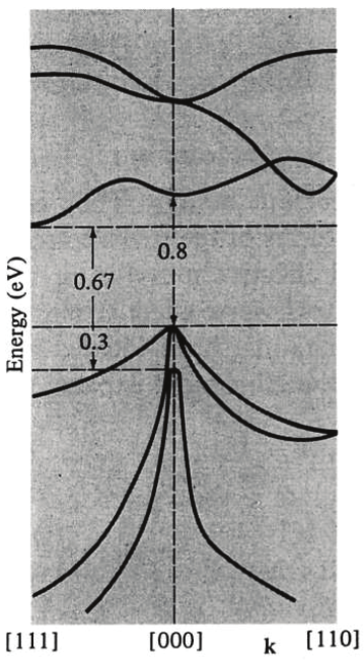
\includegraphics[height=0.5\textheight]{Figures/Electrodes/band_structure.pdf}
\caption{Scheme of the band structure in a germanium crystal.}
\label{fig:band-structure}
\end{figure}

\begin{figure}
\centering
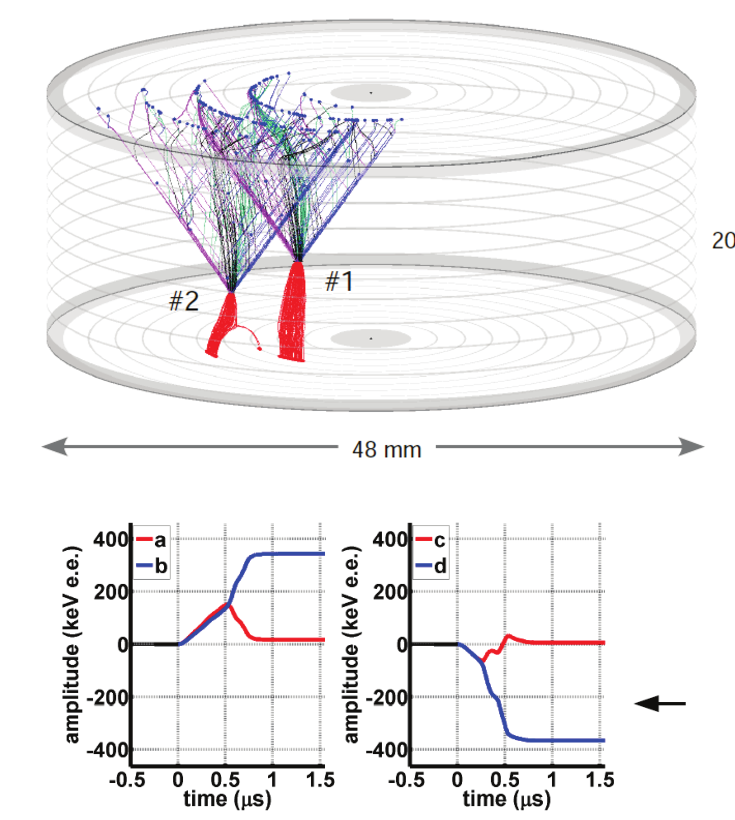
\includegraphics[height=0.5\textheight]{Figures/Electrodes/charge_drifting.pdf}
\caption{Scheme of the band structure in a germanium crystal.}
\label{fig:charge-drifting}
\end{figure}


\subsection{DAQ and electronics for ionization}
\label{par:electronics-ionization}

The electronics used for the ionization and the heat channel uses Junction Field Effect Transistor (JFET) which are operated at a low temperature of 100K inside the cryostat.
Some mumbo jumbo about the bolo-box (is it necessary ?).
The figure \ref{fig:electronics-scheme} show the scheme of the cold electronics for the heat channel (on the left) and the ionization channel (on the right).

\begin{figure}
\centering
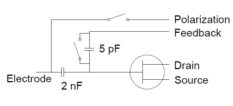
\includegraphics[width=0.48\textwidth]{Figures/Electrodes/electronic_ion_ip2i.png}
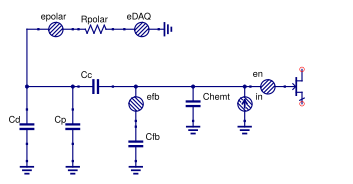
\includegraphics[width=0.48\textwidth]{Figures/Electrodes/electronic_ion_hemt.png}
\caption{Scheme of the cold electronics readout for the ionization channel currently used at IP2I (left) and in development with HEMT technology (right). One of the main difference is the floating state of the current electronic (heaviside signal) versus the polarization resistance of the HEMT (decaying exponential signal).}
\label{fig:electronics-scheme}
\end{figure}

In most experiments (source?), the ionization channel readout is done with the integration of the drifting charge current on the feedback capacitance of a charge amplifier. However, the EDELWEISS electronics directly measures the electric potential of the electrodes with a voltage amplifier. As each electrode is considered as a terminal of a capacitor $C_{electrode}$, the measured voltage is:
\begin{equation}
U = \frac{Q}{C_{electrode}}
\end{equation}
with $Q$ the drifting charge seen by the electrode.
Compare with a charge amplifier, the voltage amplifier does not involve any resistor in the amplification scheme, resulting a lower noise. However, the use of a voltage amplifier is only possible with a low leakage current, lower than 0.1fA (good for EDELWEISS, but is this possible for RICOCHET with operation on surface).

The ionization channel readout being based on the collection of electric charges, the renewal of the electric potential of the electrodes is necessary to maintain the voltage bias of the detector and to prevent the signal from leaving the readout range [-32000, +32000]. This operation, called a “reset”, consists in linking each electrodes to a polarization circuit of fixed electric potential. The linking is assured with mechanical relays (motivated by publication?) represented as a switch on the electronics scheme. The period of the resets is of a few seconds and should be adjusted empirically to the operated detectors and the event rates. In the case of surfaces operation at IP2I, the event rate is high and lot of charges are accumulated which needs for a shorter period than an underground operation at the LSM.
One should note the double switch of the mechanical relays accompanying each reset induces an artifact signal on both the heat and ionization channel. While easily discriminable from real events, these artifact signal result in dead time during which the detector is not available for valid event recording. Thus a short period of reset is not wanted.

While the majority of the electric charges produces by the ionization process are collected by the electrodes, some become trapped in the crystal (impurities) or on the surfaces of the crystal. These trapped charges are slowly accumulating and creating a counter electric field in the absorber. This results in a lower electric field perceived in the bulk of the detector which hampers a correct charge collection and decreases the sensitivity of the electrodes.
A procedure called “maintenance” is used to periodically shake up the trapped charges. These maintenances prevent, or at least slow significantly, the counter field build-up in the detector. A maintenance consists of a minute of multiples relay switches and relay changeovers. This procedure continuously invert the voltage bias in the detector, eventually destabilizing the trapped charges which are left to drift and collection in the electrodes.
During a maintenance, the detector is not available for data taking. The frequency of maintenance should be low to lower the dead time. For above ground operation, the usual maintenance period is of about 30 minutes and should be empirically adjusted to the detector and the event rate.

While a maintenance shakes up the majority of the trapped electric charges, a small fraction is not affected and participates to build up the counter field. These remaining charges are deeply trapped and need for a stronger perturbation to be freed. The detector is therefore periodically submitted to a procedure called "regeneration" aiming at a full reset of any passive electric field in the germanium crystal. With the electrodes being grounded, an intense gamma-ray radioactive source irradiates the detector. The high frequency of high energy recoils produces ionization in the whole crystal which eventually neutralize the accumulated space charges. 
As for the reset and maintenance procedures, the period between two regenerations should be empirically adjusted to the measured charge accumulation while not too frequent to avoid supplementary dead times. For above-ground operation, regeneration are realized ever two days (with a 1Cu cesium source).

Between each maintenance, the detector stays floating. The common noise can be subtracted when considering the charge conservation for all the electrodes:
\begin{equation}
\label{eq:charge-conservation}
A + B + C + D = 0
\end{equation}
With a linear combination of the raw ionization channels (A,B,C,D), we obtain new quantities (A’, B’, C’, D’) corrected from this common noise:
\begin{equation}
\label{eq:common-noise-subtraction}
A’ = \frac{3}{4} A - \frac{1}{4} \left( B + C + D \right)
\end{equation} 
The decrease of the noise level can be appreciated in the figure \ref{fig:ionization-noise} showing the noise spectrum affecting the different ionization channels before and after linear combination.

\begin{figure}
\centering
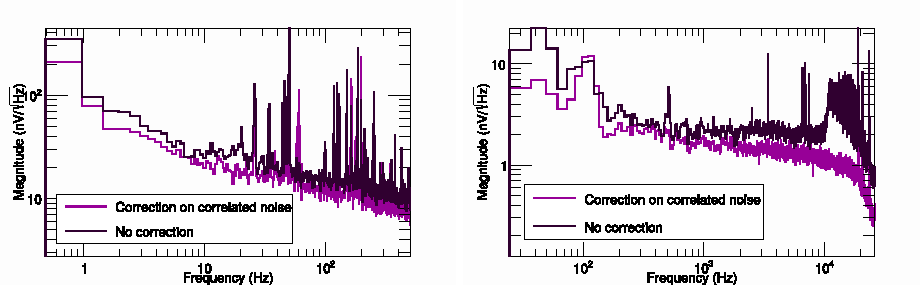
\includegraphics[width=\textwidth]{Figures/Electrodes/ionization_noise.pdf}
\caption{Average noise amplitude (in nV / Hz ) as a function of frequency of the
ionization channel for an EDELWEISS detector. The black histogram corresponds to the
noise before the correlated noise correction and the purple histogram to the noise after
the correction. Left: frequencies below 500 Hz. Right: high frequency part. [Emeline caption]}
\label{fig:ionization-noise}
\end{figure}

The ionization channel readout is sampled at an initial 100kHz. This means the period of the  measurement points is 10$\mu$s which greater than the estimated time span of an ionization signal of a few $\mu$s [ref necessary Alex.B ?]. As a result, an ionization signal is recorded as an Heaviside function. No information can be obtained on the shape of the signal.
The high readout sampling was historically chosen in EDELWEISS for the purpose of triggering on the ionization channel with a good temporal resolution (is it true ?). The highly sampled ionization signal is then averaged in order to produce a signal of frequency $f_s$ of about 400Hz. This lower sampling is able to record the information contained in the ionization Heaviside signal (its amplitude mainly) while being lightweight in term of disk space, which is essential considering the recording and processing resources at our disposal. The saved ionization signal of sampling frequency $f_s$ is composed of points which are averages of $100kHz/f_s$ points. The saved signal is therefore a skewed Heaviside-like function (more info needed? Is this work using this fact?).

{\color{blue} Discussion on the Hemt (see JB notes or Alex paper. Expected resolution and noise.}
Explaining how to propagate the noise through the hemt line (superposition theorem, thevenin-norton transformation). Presented and illustrated in the figure \ref{fig:hemt-performances}.
Simple model: Single hemt/electrode with a single detector capacitance (previously thought to be the diagonal term of the Maxwell capacitance matrix).


\begin{figure}
\centering
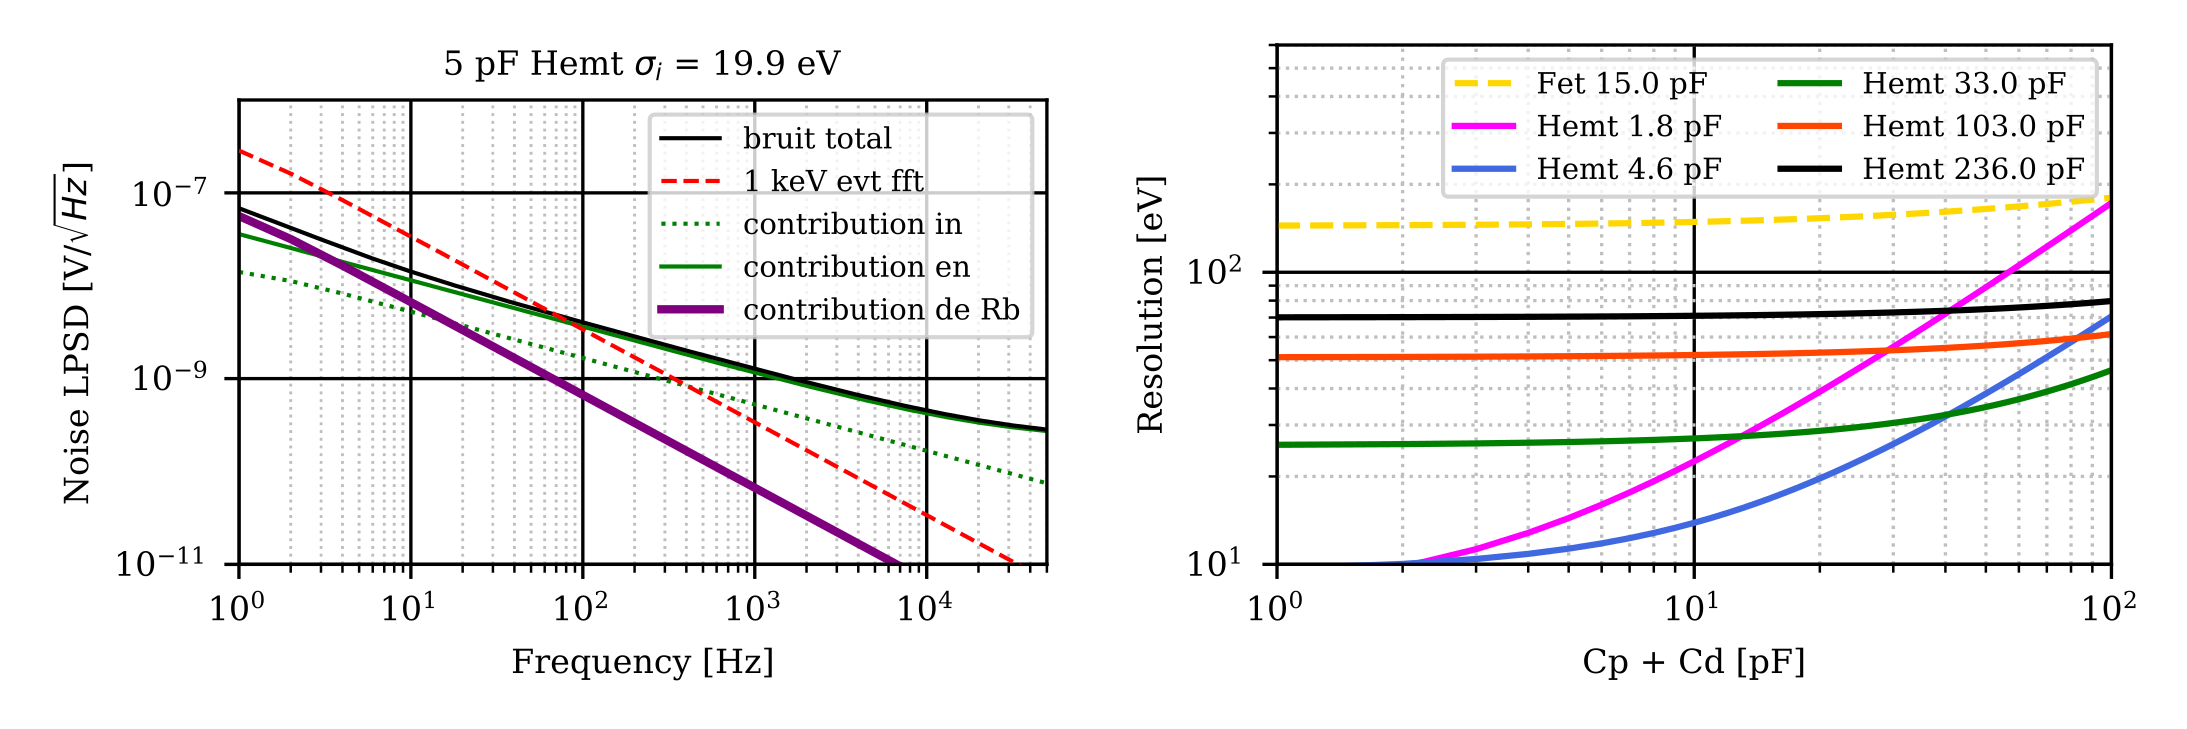
\includegraphics[width=\textwidth]{Figures/Electrodes/noise_jb.png}
\caption{Performances of the hemt technology.}
\label{fig:hemt-performances}
\end{figure}

\subsection{Aluminum Deposition}

%*Stefanos biblio here.*

The electrodes of the detectors are made by depositing aluminium on the surface of the germanium crystal. The aluminium deposition is carried out by the research group at CSNSM at Orsay. The deposition processes are still being improved.
% commet
The germanium crystal is placed in vacuum chamber where its surface is altered with beams of vaporized atoms (hydrogen, aluminium, xenon…). 
In order to prevent the surface leakage, a highly resistive layer is created under the aluminium electrodes. It is a 60 to 80 nm deep amorphous layer of hydrogenated germanium.
% test comment
Two techniques are used for the detectors presented in this work: evaporation with mask and the (photo)lithography.
A solid mask can set between the beam source and the crystal in order to shape the altered surface. In the case of concentric circular electrode, the mask (presented in figure {fig:mask-evaporation}) consists in several curved slits which allow the passage of vaporized aluminium. By rotating the mask during the process, the aluminium is deposited in a ring pattern on the germanium.
Another method to control the shape of the electrode is to use photolitography. First, the whole surface of the crystal is covered with a layer of aluminium. Then, the aluminium is coated with a chemically-protective wax. The negative of the electrode pattern is carved in the wax coating with the use of lasers (hence the name of the procedure). Once done, the germanium crystal face is immersed in chemical solution reactive with aluminium. Only the aluminium protected by the wax (patterned as the desired electrode design) is left on the surface. Finally, the wax coating is removed with an other chemical.

Advantages and Inconvenient of the 2 techniques ?
-Mask during evaporation is more precise and quicker but can only be use for simple patterns  with the cylindrical symmetry of the crystal.
-Photolitography is a longer process, and may be less precise (chemical attack of the aluminium?) but can be used for any pattern desired. Useful in the case of square grids.
- Also, some constraints on the minimum width of the electrodes ?

Leakage current exist on the surface of the crystal thanks to possible defects (ref edelweiss?). After depositing the electrodes, the bare germanium surfaces are etched with a XeF2 pulsed beam in vacuum chamber. The surface of the germanium is altered according to the following equation:
$$Ge + 2XeF_2 \longrightarrow GeF_4 + 2Xe$$
The xenon gas is removed and the fluoarated germanium surface is able to hold much higher voltage bias.

Now that the aluminium electrodes were deposited on the germanium crystal, it is possible to proceed with the cabling. The fragility of the germanium and the shallow aluminium layers motivate the use of wire-bonding as cabling technique. 

*description wire-bonding machine*

In the case of simple electrodes (full planar detector), several wires link the top (and bottom) electrodes to a conductive pad on the detector copper chassis. The conductive pad is then cabled to the ionization electronics.
With more complex design (fully interdigitized), wires are used to connect different aluminium patches, essentially imposing the same electric potential is those. With two wire bridges, It is possible to create interleaved electrodes with a biasing scheme based on the co-planar grid technique for event localisation [ref emeline 86], but more on that later.


\subsection{Luke Neganov effect}

When electric charges drift under the influence of the applied electric field in the germanium crystal, phonons are created and eventually participate to the heat signal. This process is called the Luke-Neganov [ref 63 emeline]. This phenomenon happening in semi-conductors is analogous to the Joule Effect present in conductors. 
The drifting electrons constantly dissipate their energy to the phonons bath. As the electrons stay in motion and are eventually collected by the electrodes, the electric field must provide a work $W$ compensating the energy loss going into the heat channel.
This work required for a single electron-hole pair is expressed as:
\begin{align}
W &= q_{e^{-}} \int_{ \vec{r_i} }^{ \vec{r_{e,f}} } \vec{E} d\vec{r} - q_{h^{+}} \int_{ \vec{r_i} }^{ \vec{r_{h,f}} } \vec{E} d\vec{r} \\
&=  -e \int_{ \vec{r_i} }^{ \vec{r_{e,f}} } \frac{\partial V}{\partial \vec{r}} d\vec{r} + e \int_{ \vec{r_i} }^{ \vec{r_{h,f}} } \frac{\partial V}{\partial \vec{r}} d\vec{r} \\
&= e \left( V(\vec{r_{h,f}}) - V(\vec{r_{e,f}}) \right)
\end{align}
where $q_{e^{-}} = e = - q_{h^{+}} $ represent the electric charges and $\vec{r_{i,f}}$ is the final position of the electric charge $i \in \{e^{-}, h^{+}\}$. Therefore, the energy generated by the Luke-Neganov (for a single pair) depends solely on the electric potential at the end of drift positions for the electron $\vec{r_{e,f}}$ and the hole $\vec{r_{h,f}}$.


The Luke-Neganov effect boosts the heat channel by adding a Luke-Neganov energy $E_{Luke-Neganov}$. For a recoil of type $j \in \{ e, n\}$ generating a number of electron-pairs $N^j$, the expression of this energy is:
\begin{equation}
E_{Luke-Neganov} = e \sum_{i=0}^{N^j} \left( V(\vec{r_{h,f}^i}) - V(\vec{r_{e,f}^i}) \right)
\end{equation}
A useful, and mostly accurate, approximation is to consider that all the charges end their drift by being collected at the electrodes polarized at potential $V_+$ and $V_-$. Thus, a simpler expression of the boost in energy is:
\begin{equation}
E_{Luke-Neganov} = N^j e (V_+ - V_-) = N^j e \Delta V
\end{equation}
The Luke-Neganov effect is proportional to the number of pairs $N^j$ created in the ionization process and the voltage bias $\Delta V$ of the detector. Using the equation \ref{eq:number-pairs}, we can express the boost as a function of the recoil energy $E_R$ and the associated quenching factor $Q^j$:
\begin{equation}
E_{Luke-Neganov} = Q^j \frac{E_R}{\epsilon} e \Delta V
\end{equation}
A useful simplification is to consider that $e / {\epsilon} = 1/3 \textsf{V}^{-1}$,  and to have a final expression of the Luke-Neganov boost as:
\begin{equation}
\label{eq:nl-boost}
E_{Luke-Neganov} = Q^j E_R \frac{\Delta V}{3}
\end{equation}
We see that for the same recoil energy $E_R$, an electronic recoil will benefits more than a nuclear recoil from the boost according to the comparison of  their quenching factor $Q^e > Q^n$. This is very important to keep in mind when reconstructing the recoil energy $E_R$ from the measured heat energy $E_{heat}$ as it is a function of the deposited recoil energy $E_R$ and the recoil type $j$:
\begin{align}
E_{heat} (E_R, j ) &= E_{R} + E_{Luke-Neganov} ( E_R, j) \\
&= E_R \left( 1 + Q^j(E_R) \frac{\Delta V}{3} \right)
\end{align}

*more on that now or later ? Kevee, kevnr, use of the Ei and Ec to deduce Q and Er*


\subsection{Shockley–Ramo theorem}
\label{par:shockley-ramo}

[ref quentin 100 101 102]
The signal induced on the electrodes of a detector does not corresponds to the collection of the drifting charges (when the charges reach the electrodes) but rather corresponds to the induced current starting from the moment the electron-pairs are created by a recoil. Indeed, when a charge is moving in the vicinity of an electrode, it induces an instantaneous electric current by affecting the electrostatic field lines ending on the electrode. 
[wiki after]
The Shockey-Ramo theorem states that the current $i$ induced on a given electrode due to the motion of a charge is given by:
\begin{equation}
I = E_v q v
\end{equation}
where $q$ is the charge of the particle, $v$ its velocity and $E_v$ the component of the electric field in the direction of $v$, under the following conditions: charge removed, given electrode raised to unit potential, and all other conductors grounded. This theorem ensues from Gauss theorem.
This theorem can be integrated to access the induced charge on a given electrode $k$:
\begin{equation}
\label{eq:ramo-theorem-integrated}
Q_k = - q \Phi_k(\vec{r})
\end{equation}
with $\Phi_k(\vec{r})$ the weighted potential of the electrode $k$. This weighted potential is obtained in the same conditions as $E_v$. (figure of such potential for an electrode?).
In the case of a drifting charge $q$ of initial position $\vec{r_{q,i}}$ and final position $\vec{r_{q,f}}$, the total integrated charge induced on the electrode $k$ is:
\begin{equation}
Q_k = q \left( \Phi_k (\vec{r_{q,f}}) - \Phi_k (\vec{r_{q,i}}) \right)
\end{equation}
The Shocley-Ramo theorem benefits from the superposition theorem such that it is possible to express the signal induced by a number $N$ of electron-hole pairs:

\begin{align}
Q_k &= \sum_{n=1}^{N} \left( Q_k^n(e^-) + Q_k^n(h^+) \right) \\
&= \sum_{n=1}^{N} -e \left( \Phi_k^n (\vec{r_{e,f}}) - \Phi_k^n (\vec{r_{e,i}}) \right) +e \left( \Phi_k^n (\vec{r_{h,f}}) - \Phi_k^n (\vec{r_{h,i}}) \right)
\end{align}

When considering the drifting of a single electron-hole pair, the initial position is the same for both charges and thus: $\Phi_k (\vec{r_{e,i}}) = \Phi_k (\vec{r_{h,i}})$.
The signal induced by $N$ electron-hole pairs is simplified to:

\begin{equation}
\label{eq:ramo-induced-charge}
Q_k = e \sum_{n=1}^{N} \left( \Phi_k^n (\vec{r_{e,f}}) - \Phi_k^n (\vec{r_{h,f}}) \right)
\end{equation}

It solely depends on the weighted potential of the final position of the charges. While the vast majority of charges ends up collected in the electrodes and participate with a weighted potential of $\pm 1$, some charges are trapped and so participate to the signal with the weighted potential corresponding to the position of the trap, which reduces the induced signal.
If the electrodes of the detector form a Faraday cage, all the field lines end on the electrodes and none is leaving the crystal. As a result, when considering a unique charge $q$ in the crystal, the total weighted potential $Q_T$ is:

\begin{equation}
\label{eq:charge-conservation}
Q_T = Q_A + Q_B + Q_C + Q_D = -q
\end{equation}
When considering $N$ electron-holes pairs, the Faraday cage imposes the charge conservation:
\begin{equation}
\label{eq:charge-conservation}
Q_T = Q_A + Q_B + Q_C + Q_D = \sum_{n=1}^{N} e (1 - 1) = 0
\end{equation}

Should I include the study of the trapping by Quentin ? Some studies [103 and 104 quentin ref] were done on the dependance of the electric charge  trapping in germanium crystals. Electrons are more prone to be trapped than hole. According ti Quentin, 10 to 20\% of the carriers are trapped (?). He then calculates the signal induced with trapping and also the effect of trapping as a function of the trap localization. And the impact of trapping on the heat channel.

It is now possible to know the electric charge perturbation in the detector.
In the case of the Planar38, the charges are collected by the top and bottom electrodes. We can introduce the electric charge vector associated to the Planar38:

Let's introduce the vector formalism for the electric charge $\vec{Q}$ and the electric potential $\vec{V}$ of the electrodes of a detector. Each term corresponds to a specific electrode of the detector. The Planar38 possesses two main electrodes $top$ and $bottom$. The electric charge $\vec{Q}^{PL38}$ and the electric potential vector $\vec{V}^{PL38}$ are expressed:

\begin{equation}
\vec{Q}^{PL38} =
\begin{bmatrix}
Q_{top} \\ Q_{bottom}
\end{bmatrix}
\quad
\textsf{and}
\quad
\vec{V}^{PL38} =
\begin{bmatrix}
V_{top} \\ V_{bottom}
\end{bmatrix}
\end{equation}

The FID38 possesses two main collecting electrodes $B, D$ and two veto electrodes $A, C$. The electric charge $\vec{Q}^{FID38}$ and the electric potential vector $\vec{V}^{FID38}$ are expressed:

\begin{equation}
\vec{Q}^{FID38} =
\begin{bmatrix}
Q_{A} \\ Q_{B} \\ Q_{C} \\ Q_{D}
\end{bmatrix}
\quad
\textsf{and}
\quad
\vec{V}^{FID38} =
\begin{bmatrix}
V_{A} \\ V_{B} \\ V_{C} \\ V_{D}
\end{bmatrix}
\end{equation}

With the Shockley-Ramo theorem, we can express the charge induced on the electrodes of the detectors. We consider that a recoil uses an energy $E_{Ion.}$ to create $N_p$ electron-hole pairs such that:
\begin{equation}
N_p = \frac{E_{Ion.}}{\epsilon} = \frac{E_{ion.}}{3 \textsf{eV}}
\end{equation}

We consider that the charges will drift in the crystal along the electric field lines and are not subject to trapping. All the electrons represents a total electric charge of $- N_p \cdot e$ while all the holes represents the opposite charge $N_p \cdot e$.
In the case of the Planar38 detector, the polarization scheme is usually
$$ \{top, bottom\} = \{+1V, -1V\}$$
The electrons are collected by the top electrode, while the holes are collected by the bottom electrode. The charge perturbation vector is deduced thanks to the equation \ref{eq:ramo-induced-charge}:

\begin{equation}
\label{eq:plana38-induced-charges}
\vec{Q}_{event}^{PL38} =
\begin{bmatrix}
-1 \\ 1
\end{bmatrix}
\cdot N_p \cdot e
\end{equation}

In the case of the FID38 detector, the polarization scheme is usually
$$ \{ A, B, C, D \} = \{ -0.2, +1, +0.2, -1 \} $$
Now, the electrodes upon which are collected the charges depends of the location of the recoil in the crystal. We can see on the scheme [ref scheme fid38], that the electric field forms four regions with specific collecting signatures:
\begin{itemize}
	\item bulk region, electrons collected by $B$ and holes by $D$
	\item top veto region, electrons collected by $B$ and holes by $A$
	\item bottom veto region, electrons collected by $C$ and holes by $D$
	\item equator region, electrons collected by $C$ and holes by $A$
\end{itemize}
Considering the charge collection, the FID38 thus presents four type of events with specific electric charge perturbation vectors:

\begin{equation}
\label{eq:fid38-induced-charges}
\begin{array}{rr}
\vec{Q}_{bulk}^{FID38} =
\begin{bmatrix}
0 \\ -1 \\ 0 \\ 1
\end{bmatrix}
\cdot N_p \cdot e
\quad \quad
&
\quad \quad
\vec{Q}_{veto,top}^{FID38} =
\begin{bmatrix}
1 \\ -1 \\ 0 \\ 0
\end{bmatrix}
\cdot N_p \cdot e
\\
\vec{Q}_{veto,bottom}^{FID38} =
\begin{bmatrix}
0 \\ 0 \\ -1 \\ 1
\end{bmatrix}
\cdot N_p \cdot e
\quad \quad
&
\quad \quad
\vec{Q}_{equator}^{FID38} =
\begin{bmatrix}
1 \\ 0 \\ -1 \\ 0
\end{bmatrix}
\cdot N_p \cdot e
\end{array}
\end{equation}

\subsection{Objective of the electrode study}

Produce a good design of electrodes for 32g/38g ge detectors.

Objectives:
\begin{itemize}
	\item Low capacitance
	\item High fiducial volume
	\item Good charge collection
\end{itemize}

2 Experiments : EDELWEISS and RICOCHET with different operating conditions (underground vs above ground operation, etc..)
\begin{itemize}
	\item EDELWEISS is limited by the radioactive background
	\item RICOCHET is limited by the signal-over-noise ratio
\end{itemize}


\section{Simulation for the design of the Ionization Channel}


\subsection{Introduction to Finite Element Method and Analysis:}

The simulation of the detector is done with the finite element method software COMSOL Multiphysics.
The finite element method (FEM) is the most widely used method for solving problems of engineering in fields such as structural analysis, heat transfer, fluid flow, mass transport, and increasingly more. The domain which is of interest for this work in the solving of electromagnetic potential problems.  The FEM is a particular numerical method for solving the associated partial differential equations in two or three space variables. 
To solve a problem, the FEM subdivides a large system into smaller, simpler parts that are called finite elements. This is achieved by a particular space discretisation in the space dimensions, which is implemented by the construction of a mesh of the object: the numerical domain for the solution, which has a finite number of points. Each finite elemnt is represented by a set of element equations to the original problem. The element equations are simple equations that locally approximate the original complex equations to be studied, where the original equations are often partial differential equations (PDE). The PDE is locally approximated with 
a set of algebraic equations for steady state problems (used in this work)
a set of ordinary differential equations for transient problems (not used in this work)
These equation sets are the element equations. Algebraic equation sets that arise in the steady state problems are solved using numerical linear algebra methods.
The finite element method formulation of a boundary value problem finally results in a system of algebraic equations. The method approximates the unknown function over the domain. The simple equations that model these finite elements are then assembled into a larger system of equations that models the entire problem. The global system of equations has known solution techniques, and can be calculated from the initial values of the original problem to obtain a numerical answer. It uses variational methods from the calculus of variations to approximate a solution by minimizing an associated error function. 
Studying or analyzing a phenomenon with FEM is referred to as finite element analysis (FEA). 
The subdivision of a whole domain into simpler parts has several advantages:
\begin{itemize}
	\item Accurate representation of complex geometry 
	\item Inclusion of dissimilar material properties 
	\item Easy representation of the total solution 
	\item Capture of local effects
\end{itemize}

\begin{figure}
\centering
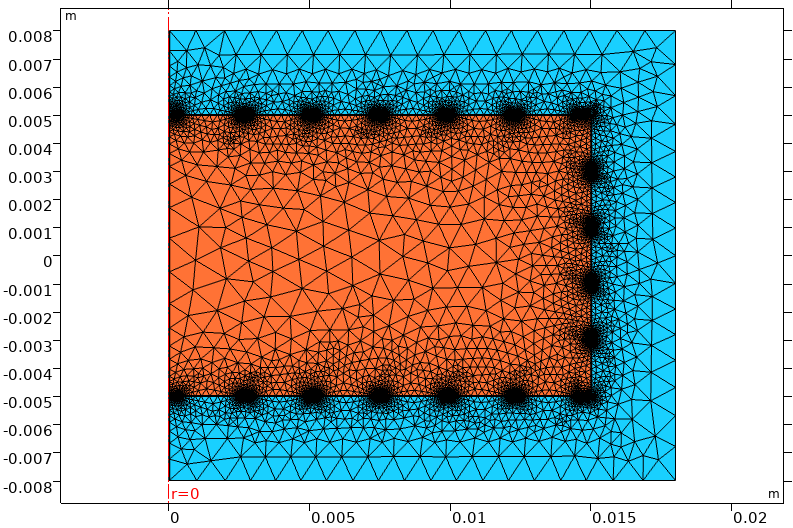
\includegraphics[width=0.48\textwidth]{Figures/Electrodes/mesh_fid38.png}
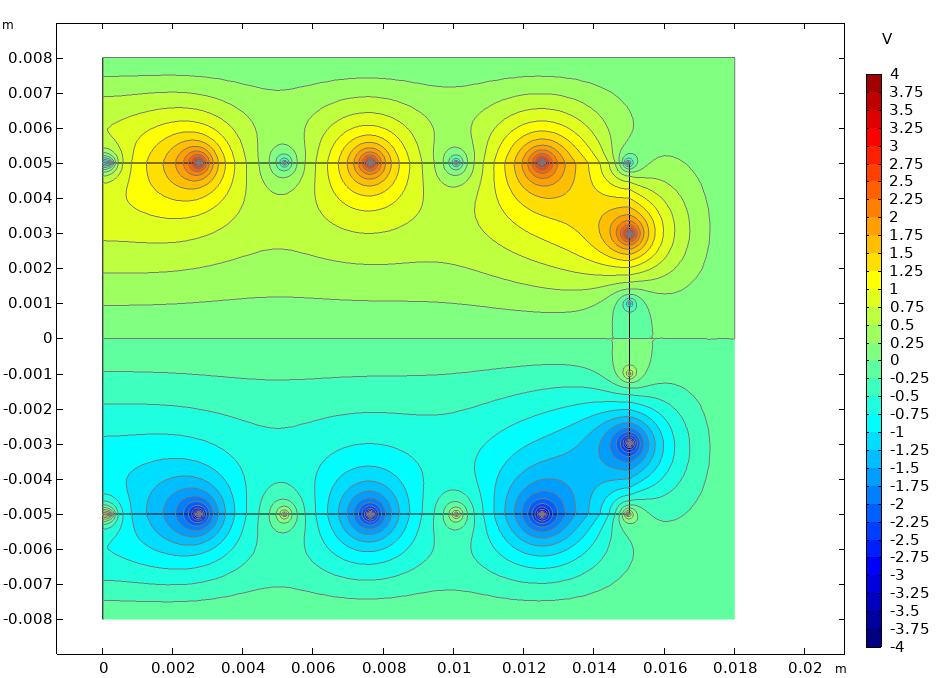
\includegraphics[width=0.48\textwidth]{Figures/Electrodes/electric_potential_fid38.png}
\caption{A small geometry, planar condensator. On left is the meshing along with the different element and materials used. On the right is the simple results of the resolution: voltage map with streamlines of the electricfield.
\textbf{Caption Left:} FEM mesh generated by the software prior to finding a solution to an electrostatic system. Two electric terminals in white (one is grounded) are facing each other separated by air in a electric floating  case. Although the geometry may seem simple, it would be very challenging to calculate the magnetic field for this setup without FEM software, using equations alone. (due to edge effects.)
\textbf{Caption Right:} FEM solution to the problem. The top and bottom electrode have electric potentials of 1V and 0V respectively. The color represents the electric potential in the air surrounding the electrodes.  The black lines represents the streamlines of the electric field in the air.  As the case is electrically floating, no streamlines can penetrate the case. We see the usual uniform electric field of a planar capacitor between the electrodes while outside the separation, the electric field is warped as it is subject to edge effects.
}
\label{fig:fid38-mesh}
\end{figure}


\subsection{Choice of the Space Dimension}

The geometry I am building. The geometry can be built in 2D-axisymmetri or 3D. A justification is needed to show that 2D is good enough for the study. Because the calculation are much quicker with it and better for a quick modelization.
The Comsol software propose several choices of space dimension for the modelization. The most evident would be to work with a 3D model of the detectors. However, it is possible to benefit from the natural cylindrical symmetry of the detectors in this study to ease the calculation. Indeed, solving the electric equations on the whole volume would be redundant as it can be done a radial slice of the detector and then revolved around its central axis. Working with this radial slice of a system is using a space dimension called the 2D-axisymmetry in COMSOL.

\begin{figure}
\centering
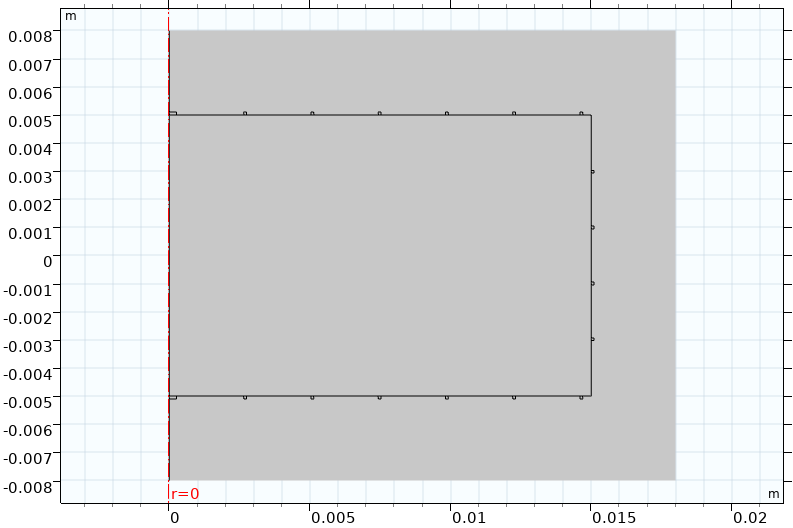
\includegraphics[width=0.48\textwidth]{Figures/Electrodes/geometry_2d.png}
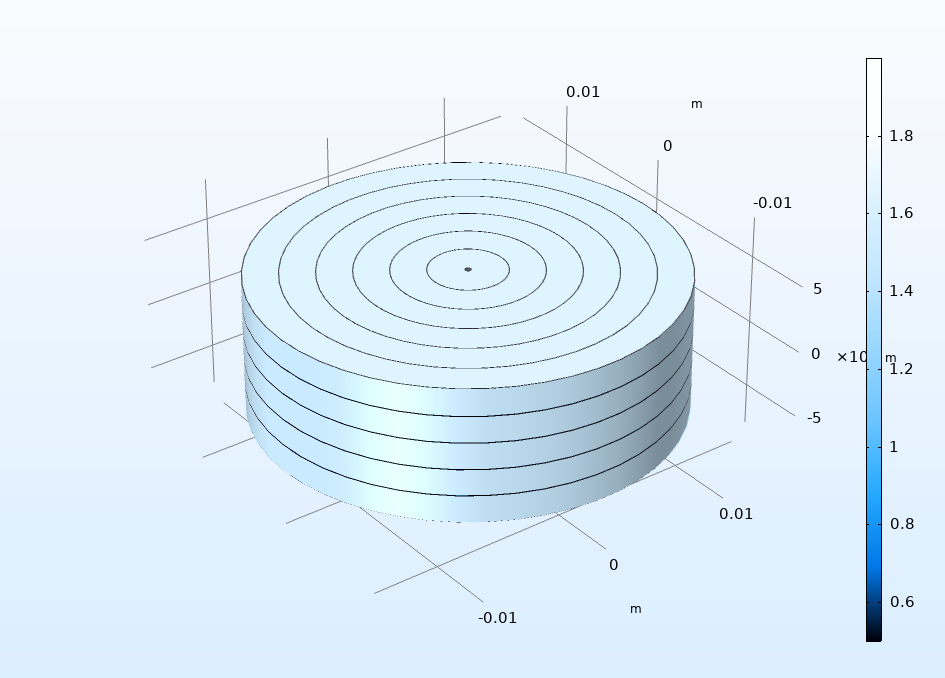
\includegraphics[width=0.48\textwidth]{Figures/Electrodes/detector_3d.png}
\caption{
A geometry in 2D-axisymmetry and in 3D. On the left, the geometry is built on a plane (in two dimensions) and around the axis of symmetry situated at r=0. The germanium crystal (inner rectangle) is equipped with electrodes on each planar face, and is installed is a copper chassis (outer ractangle) where the air was vaccumed.
The same geometry can be obtained with a 3D modelization, without taking into account the symmetry of the system. As a result, a more complex meshing is needed to solve the problem which translate to a longer calculation time. However, it is possible to add non-symmetric features such as non-centered rectangular NTD, or the wire-bonding bridge between the electrodes (not featured in this study). 
}
\label{fig:space-dimension-geometry}
\end{figure}

The figure [fig] presents the modelization of a the same detector using both space dimension. It was checked (justification needed) that both space dimension result in the same solutions. (variations between the two are negligible). The advantage of the 2D-axisymmetry lies in the solving of the electric equations in a 2D plane with pertinent variable changes to consider the axisymmetry. This needs for a simple 2D meshing. On the contrary the 3D modelization do not benefit from the symmetry and solve the equations in the whole volume. This requires a more complex meshing with more vertexes (number?). The calculation time is therefore longer. However, when adding non-symmetrical features to the system, the 3D modelization is the only way to solve the equations with a precise geometry. Non-symmetrical features can be the NTD thermal sensor, the wire-bond bridge cabling the electrodes or even the Teflon pad fixing in place the germanium crystal in the copper chassis.
As this work aims at studying multplie geometry by scanning over different parameters, the 2D-axisymmetry was chosen in order to have short calculation times. The 3D might be used specifically to determine the influence of additionnal features. (Bonus study if time ?)


\subsection{Meshing choice}
\label{par:mesh-scale}

When solving a problem with the finite element method, the choice of the meshing is essential. As the FEM is essentially approximating the analytical solution with a numerical approach over the vertexes, the meshing should be well constructed to assure a precise simulation. For a given physic system, the analytical solution can be more precisely approximate as the number of vertexes is increased. However, a high number of vertexes induces an equal number of local numerical solving. COMSOL propose a automatic optimization of the meshing which adapts the size of meshing to the geometry of the system. With this optimized meshing, there are a lot of vertexes near small geometric features assuring that a rapidly varying electric field is correctly mapped. At the same time, there are only few vertexes at location where the electric field is almost uniform. This optimization of the meshing is possible with the “Physics-based” option of COMSOL which still accept a mesh scale parameter. Simulation of the reference designs Planar38 and FID38 were ran with different mesh scales and the results are presented in the table \ref{tab:mesh-scale}. There are nine mesh scales proposed by COMSOL, starting from the "Extremely Coarse" scale with a low number of simplex, a low accuracy and very quick run time, and continuing with increasingly refined scale to the "Normal" scale, which should result in a trade-off between simulation time and precision, eventually reaching the "Extremely Fine" scale with a very high precision obtained after a long calculation time. As expected, the more refined the scale is and the more triangles are used for the simulation (except for Extremely Coarse, maybe it is a non-optimized mesh generating algorithm in use). As the FID38 design has more electrodes of small size than the other Planar38 design, the mesh is generated with more simplex. It is consistent with the fact that the simulation of the Planar38 design run quicker than for the FID38.
In order to estimate the accuracy of the simulation scanning over the different scales, a capacitance value corresponding to the first diagonal term of the Maxwell capacitance matrix (see the later paragraph \ref{par:capacitance-matrix}) is evaluated. Additionally, a percentage of the relative error on the capacitance calculation is calculated. The capacitance of the "Extremely Fine" scale is chosen to be the reference for this relative error. Thus, by definition, the relative error of the "Extremely Fine" is zero. The table \ref{tab:mesh-scale} shows that as the scale is more refined, the capacitance is getting closer to the reference capacitance.
In the case of the Planar38, the relative error starts at 0.78\% and eventually reaches zero for the "Normal" scale. Concerning the FID38 design, the relative error is greater for all scales compared to the Planar38. This may be due to the more complex geometry. Although the error is superior to 1\% for the less refined scales, from the "Normal" scales the error is inferior to 0.1\%.
Considering that the "Normal" and "Fine" possesses a similar number of simplex and runtime, the simulation presented in this work are ran with the "Fine" scale. The capacitance calculation are affected by a relative error of about 0.1\%. 

\begin{table}[]
\centering
\resizebox{\textwidth}{!}{%
\begin{tabular}{c|rrr|rrr}
\multirow{2}{*}{Mesh Scale} & \multicolumn{3}{c|}{Planar38} & \multicolumn{3}{c}{FID38} \\ \cline{2-7} 
 &
  \multicolumn{1}{c}{\# Triangles} &
  \multicolumn{1}{c}{Capacitance {[}pF{]}} &
  \multicolumn{1}{c|}{Relative Error {[}\%{]}} &
  \multicolumn{1}{c}{\# Triangles} &
  \multicolumn{1}{c}{Capacitance {[}pF{]}} &
  \multicolumn{1}{c}{Relative Error {[}\%{]}} \\ \hline
Extremely Fine              & 37837    & 14.923   & 0      & 106028   & 19.217  & 0     \\
Extra Fine                  & 11721    & 14.923   & 0      & 41991    & 19.223  & 0.03  \\
Finer                       & 6306     & 14.923   & 0      & 29996    & 19.222  & 0.02  \\
Fine                        & 4368     & 14.923   & 0      & 22504    & 19.232  & 0.08  \\
Normal                      & 4258     & 14.923   & 0      & 22340    & 19.232  & 0.08  \\
Coarse                      & 2472     & 14.924   & 0.01   & 15288    & 19.263  & 0.24  \\
Coarser                     & 1303     & 14.934   & 0.07   & 7596     & 19.475  & 1.34  \\
Extra Coarse                & 1260     & 14.964   & 0.27   & 7915     & 19.693  & 2.47  \\
Extremely Coarse            & 1937     & 15.037   & 0.76   & 19714    & 19.625  & 2.12 
\end{tabular}%
}
\caption{Scanning the mesh scale of the simulated Planar38 and FID38 design. The control values are the number of triangles in the mesh, the first diagonal term of the Maxwell capacitance matrix and the relative error on the capacitance calculation with the "Extremely Fine" scale chosen as reference.}
\label{tab:mesh-scale}
\end{table}

\subsection{Modelization of a RED detector}

This work aims at discovering and quantifying the impact of the design of the electrodes upon the ionization channel performance. Multiple geometries were simulated with common parameters and sometimes their own specific parameters. As a result, the study of the common parameters is illustrated with a reference electrode geometry “FID38”, and the impact of specific parameters are discussed with their associated geometry.
The “FID38” geometry stands for a detector composed of a 38g germanium crystal with Fully InterDigitized (FID) electrodes. The absorber is simulated as a cylinder of height 10mm and radius 15mm composed of germanium crystal of relative electric permittivity 16.3. It is surrounded by a cylindrical copper chassis leaving a distance $d_{chassis}=3mm$ between the chassis and the surface of the absorber. The copper chassis is electrically grounded at a potential $V_chassis=0V$. It is assumed that the influence of the Teflon clamps holding the absorber is negligible considering their size and the low relative electric permittivity of the material ($\epsilon_r=2.1$). As such, Teflon clamps are ignored in the simulation. The space between the germanium crystal and the copper chassis is considered to be vacuum of relative permittivity 1. The electrodes are simulated by extruded annuli, resembling thin rings, composed of aluminium of height $h_{Al}=0.01[mm]$ and width $w_{Al}=0.08mm$. Real electrodes possess a much lower height of about 50nm. However, this value is so low that the meshing is invariably messed up. For a FID geometry, there are 4 electrodes labeled ‘A’, ‘B’ ‘C’, and ‘D’ composed of multiple rings linked by wire-bound bridges. Inside COMSOL, multiple electrodes can be assigned to the same electric terminal, which means that they are electrically linked and share their potential and charges. It is therefore possible to avoid the simulation of the wire-bonding bridges between the different FID rings. (at least for now, see later in bonus study if it is really impacting something). Each physical electrodes ‘A’, ‘B’, ‘C’, ‘D’ represented by terminals in COMSOL are polarized at a fixed voltage $V_i \, \textsf{with} \, i \in {A,B,C,D}$. The terminals ‘B’ and ‘D’ corresponds to the main electrodes, labeled “Collect”, which collect the electric charges produced in the bulk of the detector. The terminal ‘A’ and ‘C’ corresponds to auxiliary electrodes, labeled “Veto”, which collect the charges produces near the surface of the absorber. The polarization of the electrodes is controlled by three parameters :
\begin{itemize}
	\item $V_{bias}=8V$, which is the main voltage bias of the detectors
	\item $R_{veto}=-0.25$, which is the ratio of the voltage bias of the veto electrodes over the main voltage bias
	\item $S_{bias}=0.5$, varying between 0 and 1, it represents the vertical symmetry of the polarization.
\end{itemize}
With this three parameters, the fixed voltage of the terminals are:
\begin{equation}
\label{eq:fid-polarization}
\begin{array}{l c c c S r}
V_B &=& V_{bias} \times S_{bias} &=& \num{1} & \si{\volt} \\
V_D &=& - V_{bias} \times (1 - S_{bias}) &=& \num{-1} & \si{\volt} \\
V_A &=& V_{bias} \times \left( S_{bias} - \frac{\left( 1 + R_{veto}\right)}{2}\right) &=& \num{-0.25} & \si{\volt}  \\
V_C &=& V_{bias} \times \left( S_{bias} + \frac{\left( -1 + R_{veto}\right)}{2}\right) &=& \num{0.25} & \si{\volt} 
\end{array}
\end{equation}

Several parameters govern the location of the ring-shaped electrodes on the top and the lateral surface of the absorber. The number of total concentric electrodes on the top (resp. lateral) surface is $n_{top}=7$ (resp. $n_{lateral}=2$). The distance separating the center of each top (resp. lateral) electrode is $d_{Al}^{top}=2.395mm$ (resp. $d_{Al}^{lateral}=1.98mm$). The innermost and outermost top electrodes are assigned to the veto terminals ‘A’ or ‘C’. The radius of the innermost electrode is $r_{inner}=0.25mm$. The radius of the outermost is limited to the radius of the germanium crystal minus a band of width $r_{edge}=0.3mm$. This comes from the limits of the aluminium deposition technique employed: it is not possible to have a thin aluminium electrode at less than $0.3mm$ from the edge of the top surface of the germanium crystal. The two most centered lateral electrodes are also assigned to the veto Terminals ‘A’ and ‘C’. These electrodes are distant from the equatorial line of the crystal by $d_{equatorial}=1mm$.

\begin{figure}
\centering
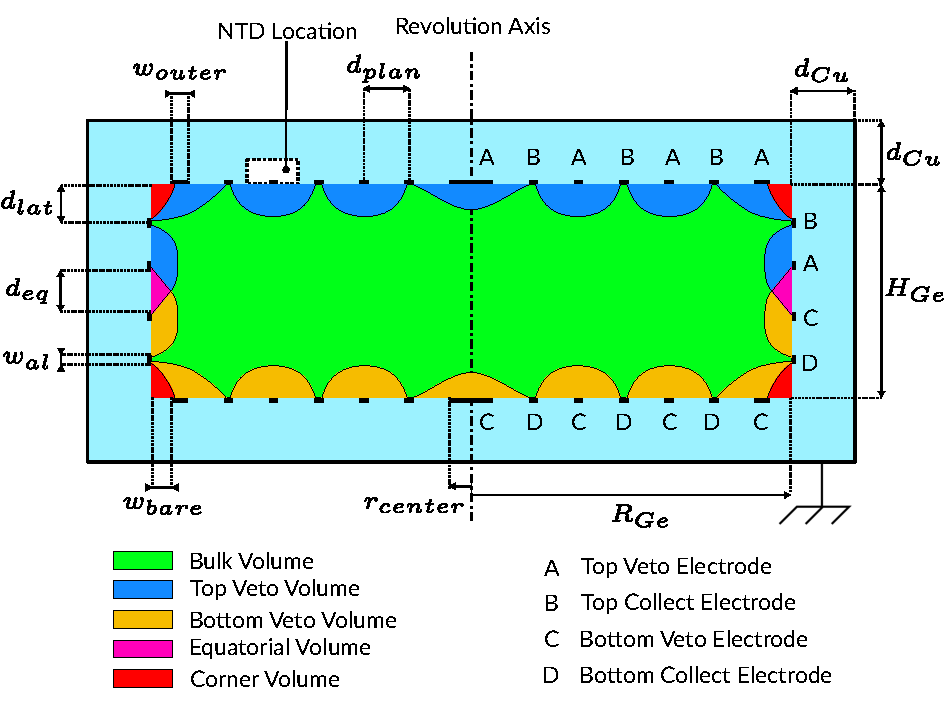
\includegraphics[scale=1]{Figures/Electrodes/scheme_fid38.pdf}
\caption{
Scheme of the FID38 design.
}
\label{fig:fid38-scheme}
\end{figure}

\begin{figure}
\centering
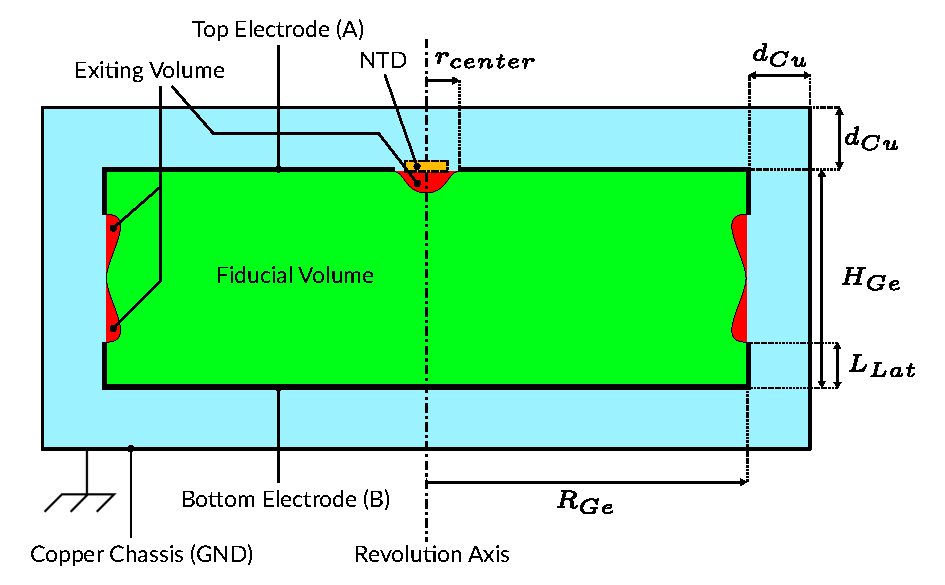
\includegraphics[scale=1]{Figures/Electrodes/scheme_pl38.pdf}
\caption{
Scheme of the PL38 design.
}
\label{fig:pl38-scheme}
\end{figure}


The electric equations are solved only in the insulators domains : the germanium absorber and the surrounding vacuum inside the copper chassis. The aluminium electrodes are set to a fixed potential and their interior is excluded from the simulation. 

\begin{table}[]
\centering
%\resizebox{\textwidth}{!}{%
\begin{tabular}{l c S}
Parameter                                   & Symbol        & {Default Value} \\ \hline \hline
Ge crystal Height                           & $H_{Ge}$      & \SI{10}{\mm}  \\
Ge crystal Radius                           & $R_{Ge}$      & \SI{15}{\mm}    \\
Distance between crystal and copper chassis & $d_{Cu}$      & \SI{3}{\mm}     \\
Electrode Thickness                         & $h_{Al}$      & \SI{1}{\micro\meter}   \\
Electrode Width                             & $w_{Al}$      & \SI{80}{\micro\meter}  \\
Radius of the innermost planar electrode    & $r_{center}$   & \SI{0.25}{\mm}   \\
Width of bare Ge crystal on corners      & $w_{bare}$    & \SI{0.3}{\mm}  \\
Width of the outermost veto electrode    & $w_{outer}$    & \SI{0.08}{\mm}  \\
Number of planar electrodes                 & $n_{plan}$  & {$7$}             \\
Number of lateral electrodes                & $n_{lat}$ & {$2$}             \\
Interdistance of Planar electrodes          & $d_{plan}$  & \SI{1.98}{\mm}  \\
Interdistance of Lateral electrodes         & $d_{lat}$ & \SI{2.40}{\mm}  \\
Equatorial distance & $d_{eq}$ & \SI{2}{\mm}  \\
Main Voltage Bias                           & $V_{bias}$    & \SI{2}{\volt}      \\
Ratio Veto/Main voltage bias                & $R_{veto}$    & {$-0.25$}         \\
Symmetric factor of the voltage bias        & $S_{bias}$    & {$0.5$}         
\end{tabular}
%}%
\caption{List and Value of the default parameters for the FID38 design.}
\label{tab:fid38-default-parameters}
\end{table}

\begin{table}[]
\centering
%\resizebox{\textwidth}{!}{%
\begin{tabular}{l c S}
Parameter                                   & Symbol        & {Default Value} \\ \hline \hline
Ge crystal Height                           & $H_{Ge}$      & \SI{10}{\mm}  \\
Ge crystal Radius                           & $R_{Ge}$      & \SI{15}{\mm}    \\
Distance between crystal and copper chassis & $d_{Cu}$      & \SI{3}{\mm}     \\
Electrode Thickness                         & $h_{Al}$      & \SI{1}{\micro\meter}   \\
Radius of the central NTD hole    & $r_{center}$   & \SI{1.5}{\mm}   \\
Corner length & $L_{lat}$ & \SI{2}{\mm}  \\
Main Voltage Bias                           & $V_{bias}$    & \SI{2}{\volt}      \\
Symmetric factor of the voltage bias        & $S_{bias}$    & {$0.5$}         
\end{tabular}
%}%
\caption{List and Value of the default parameters for the PL38 design.}
\label{tab:pl38-default-parameters}
\end{table}


\subsection{Stationnary Study}

The stationary study consists in solving the electrostatic equations for the given parameters and voltage bias. The FEM solution consists in the electric potential value for each vertex of the mesh. This values are interpolated and used to represent the potential on a radial slice of the detector (as seen in figure [fig potential]). It is possible to apply a gradient function to obtain the electric field in the detector (as seen in figure \ref{fig:fid38-enorm}) along with the streamline of the electric field. The streamlines are useful to visualize the direction of the electric field in the crystal and predict the trajectory of the drifting charges in the detector.

The electric potential is presented on the right figure \ref{fig:fid38-mesh} and the electric field norm is presented on the left figure \ref{fig:fid38-enorm} along with the streamlines. As expected from a FID design, the electric potential is rapidly changing near the electrodes in order to shape the electric field which is thus rather high near the electrodes. The streamlines shows the expected trajectories for the drifting charges and thus the collecting electrodes for each type of recoils. In the bulk of the crystal, the electric field is quite uniform although it suffers from a loss in intensity due to the influence of the veto electrodes. Concerning the norm of the electric field, we observe that the veto electrodes are creating low-norm regions (in black on figure \ref{fig:fid38-enorm}) at the frontier between the veto and the bulk region. Event though these low-norm regions could increase the chance of trapping or unwanted recombination, we note that streamlines are diverging from these regions.

In order to monitor the norm of the electric field in the whole crystal, its volumetric density is recorded and presented on the right figure \ref{fig:fid38-enorm}. The majority of the crystal seems to be subject to a electric field of norm $\approx 200 V/cm$. Each peak can be link to specific region in the crystal with equal norm. The low-norm regions appears to be negligible in proportion.

\begin{figure}
\centering
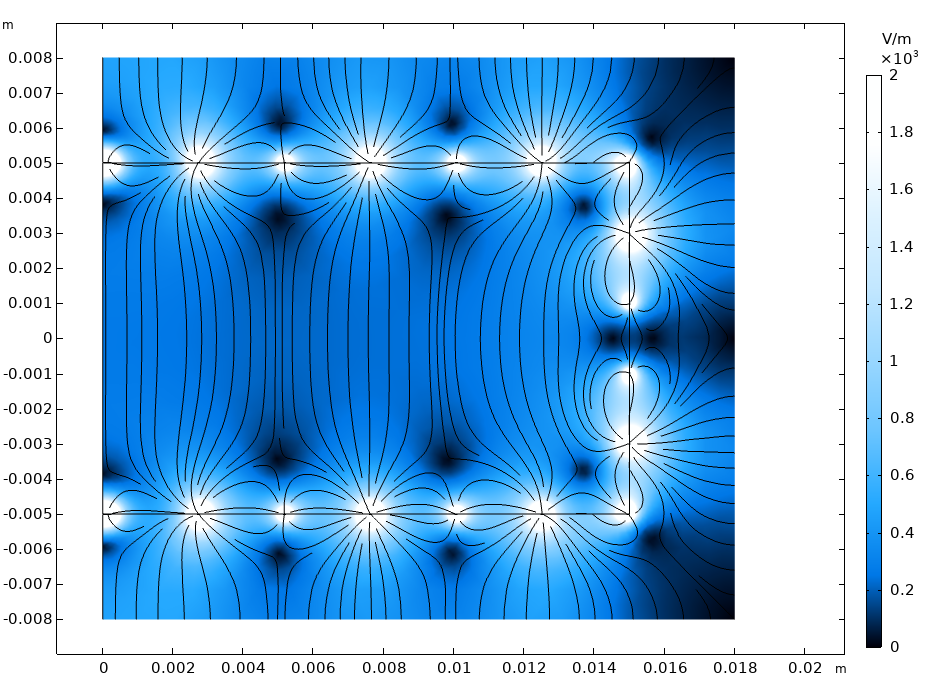
\includegraphics[width=0.48\textwidth]{Figures/Electrodes/electric_field_norm.png}
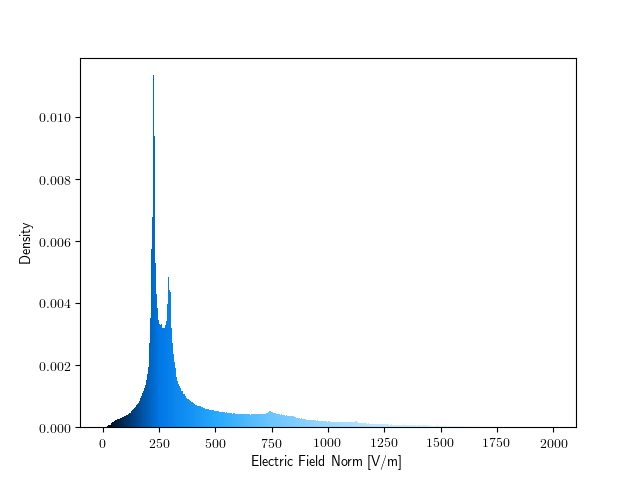
\includegraphics[width=0.48\textwidth]{Figures/Electrodes/hist_enorm.png}
\caption{
\textbf{Left:} Graph of the norm of the electric field in the detector with streamlines.
\textbf{Right:} Density Histogram of the electric field norm value in the partitioned volume of the Ge crystal.(need image annotation, on the different peak in particular)
}
\label{fig:fid38-enorm}
\end{figure}

\begin{figure}
\centering
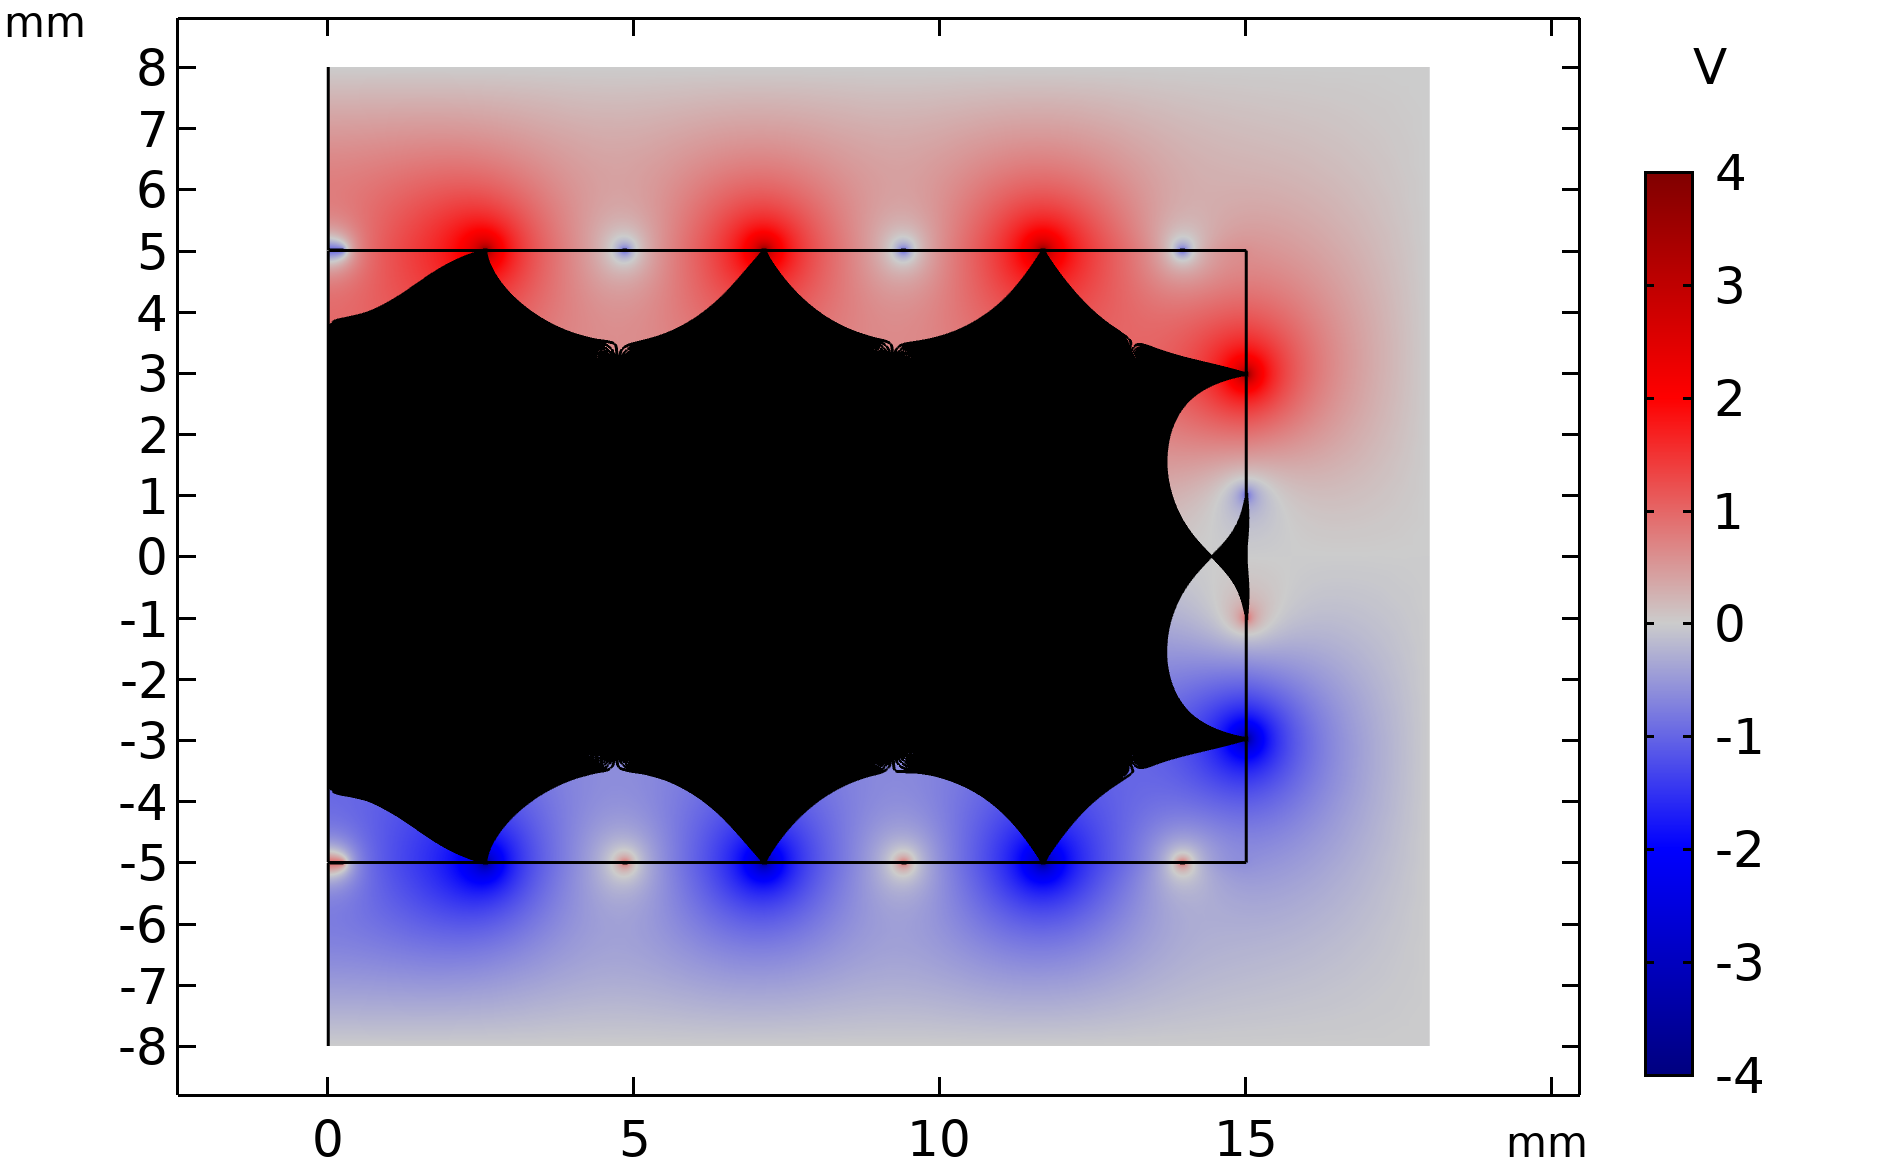
\includegraphics[width=0.48\textwidth]{Figures/Electrodes/fid38_fiducial_streamlines.png}
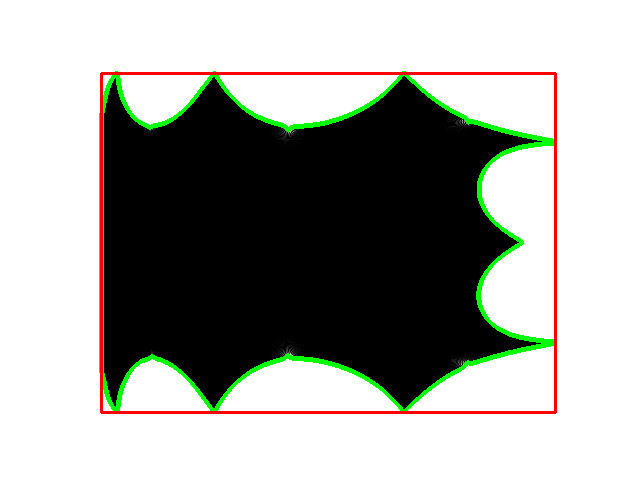
\includegraphics[width=0.48\textwidth]{Figures/Electrodes/fid38_fiducial_contour.png}
\caption{
\textbf{Left:} Graph of the electric potential with fiducial streamlines in FID38.
\textbf{Right:} Total(red) and Fiducial(green) volume contours after processing of the streamlines crossing z=0. Compared to the original graph on the left, the streamlines are stretched towards the exterior of the cylindrical Ge crystal according to a linear scaling with the radius of the point. This scaling emulates the volume of a cylinder in a 2D plan.
}
\label{fig:fid38-fiducial}
\end{figure}

\label{par:fiducial-volume}

The left figure \ref{fig:fid38-fiducial} presents the streamlines in the crystal with controlled starting points with a height set at 0 (starting from the middle of the crystal). These streamlines belongs to the bulk region and equatorial regions. With some processing, it is possible to discard the streamlines linking two veto electrodes and to keep only a contour of the fiducial streamlines. A correction taking into account the revolution of the 2d-axisymmetry is needed to calculate volumes. The right figure \ref{fig:fid38-fiducial} presents the fiducial contour (in green) and a whole crystal contour (in red) proportionnal to the fiducial and crystal volume. Graphically comparing the area of the two contours yields the fiducial volume fraction of the detector. With default parameters, The FID38 design has a fiducial volume fraction of 69.5\%. Also with default parameters, the Planar38 has a fiducial volume fraction of 98\%.


\subsection{Weighted Potential Study}
\label{par:weighting-potential}

This paragraph is linked to a previous one introducing the signal generation on the electrodes by drifting electric charges with the Shockley-Ramo theorem. A map of the weighted potential associated to each electrode is obtained by fixing the potential of the considered electrode to the unitary value of 1V and grounding all the other terminals. (see left of  figure [Weighted potential]). The total weighted potential is obtained by summing over the different electrodes. (see left of  figure [Weighted potential]).

\begin{figure}
\centering
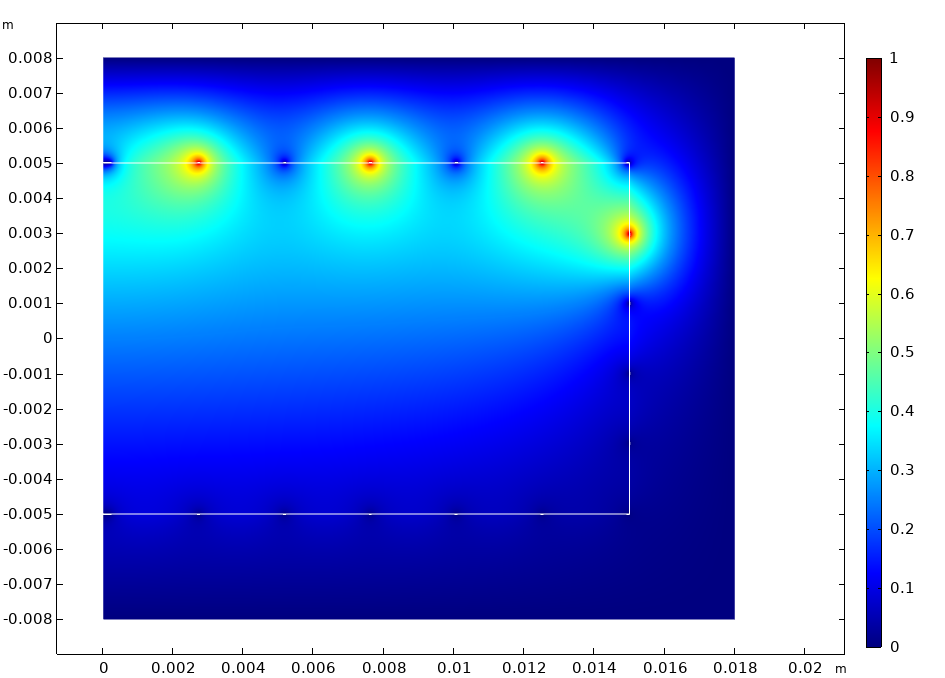
\includegraphics[width=0.48\textwidth]{Figures/Electrodes/weighted_potential_collect.png}
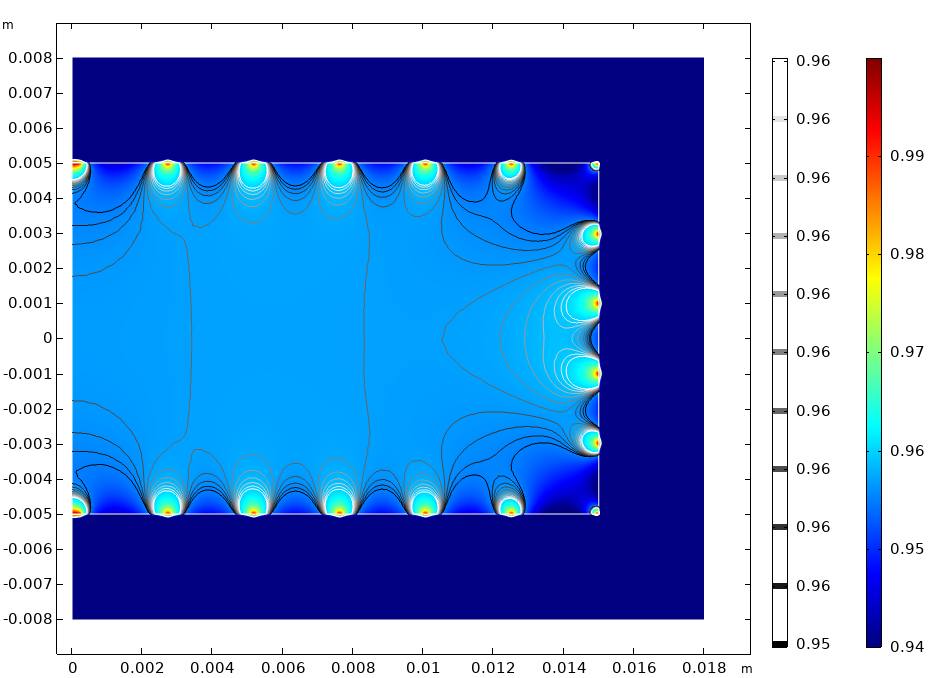
\includegraphics[width=0.48\textwidth]{Figures/Electrodes/weighted_potential_total.png}

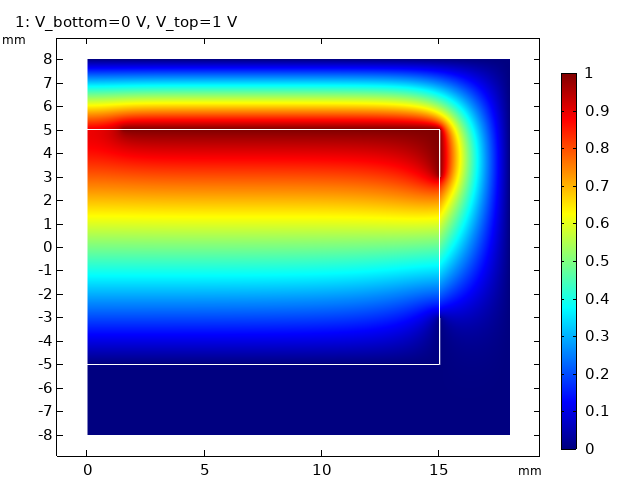
\includegraphics[width=0.48\textwidth]{Figures/Electrodes/weighted_potential_top.png}
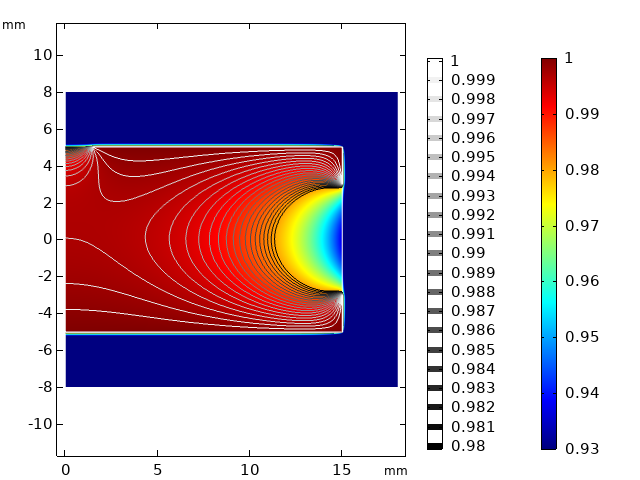
\includegraphics[width=0.48\textwidth]{Figures/Electrodes/weighted_potential_total_planar38.png}


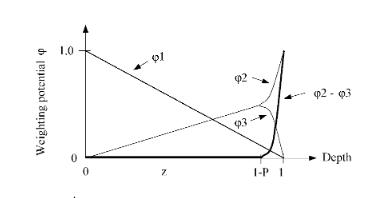
\includegraphics[width=0.48\textwidth]{Figures/Electrodes/ramo_potential.png}
\caption{
\textbf{Top Left:} Graph of the weighting potential for the main top collect electrode, for the FID38 design.
\textbf{Top Right:} Graph of the total weighting potential. It corresponds to the sum of the weighting potential of all the electrodes, for the FID38 design.
\textbf{Center Left:} Graph of the weighting potential for the main top collect electrode, for the Planar38 design.
\textbf{Center Right:} Graph of the total weighting potential. It corresponds to the sum of the weighting potential of all the electrodes, for the Planar38 design.
\textbf{Bottom Center:} Graph of the weighting potential of different electrodes as a function of the position in the crystal.
}
\label{fig:weighting-potential}
\end{figure}

While the red color indicate a total weighted potential $\phi_T$ which tends to 1, the color blue is associated to an inferior total weighted potential. We see that the potential is almost uniform in the bulk of the crystal while it is increasing near the electrodes. According to the Shockley-Ramo theorem, electron-holes pairs created very near an electrode are inducing a signal almost entirely in the A,B,C,D electrode. However, for pairs created in the bulk of the crystal, a fraction (1-0.96=0.04=4\%) of the signal is induced in the copper chassis outside of the crystal. As a result, the detector is not a perfect Faraday Cage, but is approaching its properties as the minimum total weighted potential in the crystal is 0.94.  

{ color{blue} Discussion on the loss of energy in the case of trapping as a result of a total weighted potential inferior to 1. Rough estimation of the limit on the intrinsic resolution of the ionization resolution for several fraction of trapping per recoil.}

For the Planar38 design, the average total weighted potential in the crystal is 98\%

\subsection{Capacitance calculation with the Source Sweep Study}
\label{par:capacitance-matrix}

The sensitivity of the ionization channel is inversely proportional to the capacitance of the electrodes. Therefore, the capacitance is a performance indicator for the different design of electrodes.
The common form of a capacitance is a parallel-plate capacitor: two conductive plates separated by a dielectric material of relative electric permittivity $\epsilon_r$. For the ideal case of this system, the capacitance $C$ is proportional to the surface area of the electrodes $A$ and inversely proportional to the distance between the terminals $d$ such that:
\begin{equation}
C = \epsilon_0 \epsilon_r \frac{A}{d}
\end{equation}
For this system composed of only two electrodes, the capacitance $C$ governs the amount of electric charges on the plates $Q$ and $-Q$ necessary to impose a voltage $V$ between them according to the equation:
 \begin{equation}
 \label{eq:capacitance-definition-simple}
C = \frac{Q}{V}
\end{equation}
In the case of germanium bolometers, the capacitance is more complex as it takes into accounts the grounded copper chassis, two main collecting electrodes and, depending on the considered design, two auxiliary electrodes (guard or veto). The previous equation does not apply in system with more than two terminals and should be generalized to any electric system with a number $N$ of electrodes. For such a system, the charge and electric potential of all the electrodes are represented by the the charge vector $\vec{Q}$ and the potential vector $\vec{V}$ as:

\begin{equation} 
\label{eq:vector-charge-potential}
\vec{Q} = 
\begin{pmatrix}
Q_{1} \\ 
Q_{2} \\ 
\vdots \\ 
Q_{N}
\end{pmatrix} 
\quad \textsf{and} \quad
\vec{V} = 
\begin{pmatrix}
V_{1} \\ 
V_{2} \\ 
\vdots \\
V_{N}
\end{pmatrix} 
\end{equation}

In order to generalize the calculation of the capacitance to the electrodes of the bolometer, the concept of Maxwell capacitance matrix $\bm{C}$ is introduced:

\begin{equation} 
\label{eq:maxwell-capacitance-matrix}
\bm{C} = 
\begin{pmatrix}
C_{11} & C_{12} & \cdots & C_{1N} \\ 
C_{21} & C_{22} & \cdots & C_{2N} \\ 
\vdots & \vdots & \ddots & \vdots \\ 
C_{N1} & C_{N2} & \cdots & C_{NN}
\end{pmatrix}
\quad \textsf{with} \quad
\bm{C}_{ij} = \frac{\partial Q_i}{\partial V_j}
\end{equation}

This matrix describes the relation between the charge $Q_i$ and the voltage $V_i$ of all the conductors in the system, and generalize the \ref{eq:capacitance-definition-simple} as:

\begin{equation} 
\label{eq:capacitance-definition-matrix}
\vec{Q} =
\bm{C} \vec{V}
\quad \Leftrightarrow \quad
\vec{V} =
\bm{C}^{-1} \vec{Q} = \bm{P} \vec{Q}
\end{equation}
with $\bm{P}$ being the inverse of the Maxwell capacitance matrix named the elastance matrix. Its terms $\bm{P}_{ij}$ are called the coefficients of potential such that:
\begin{equation}
\label{eq:elastance-matrix}
\bm{P} =
\begin{pmatrix}
P_{11} & P_{12} & \cdots & P_{1N} \\ 
P_{21} & P_{22} & \cdots & P_{2N} \\ 
\vdots & \vdots & \ddots & \vdots \\ 
P_{N1} & P_{N2} & \cdots & P_{NN}
\end{pmatrix}
\quad \textsf{with} \quad
\bm{P}_{ij} = \frac{\partial V_i}{\partial Q_j}
\end{equation}
It was demonstrated [ref?] that the coefficients of potential are symmetrical such that  $\bm{P}_{ij} = \bm{P}_{ji}$ which induces that the Maxwell capacitance matrix is symmetric as well.

A key observation when comparing the two-plates capacitance equation \ref{eq:capacitance-definition-simple} to the multiple plates capacitance equation \ref{eq:capacitance-definition-matrix} is that the electric charge $Q_i$ and potential $V_i$ of a given electrode $i$ are no longer proportional with multiple plates. With the generalized view, adding a charge on a single electrode changes the potential of all the electrodes in the system.

While the Maxwell capacitance matrix is useful to study the generation of signal from charge collected by the electrodes with the equation \ref{eq:capacitance-definition-matrix}, there are no readily available interpretation for its term. An alternative to the Maxwell capacitance matrix is the mutual capacitance matrix $\bm{C}^m$. This terms of the mutual capacitance terms hold the benefit of being easily illustrated as lumped capacitance between the electrodes of a system. The figure [scheme mutual capacitance] presents a scheme of the four electrodes of the FID38 design in the grounded copper chassis.

\begin{figure}
\begin{minipage}{0.58\textwidth}
    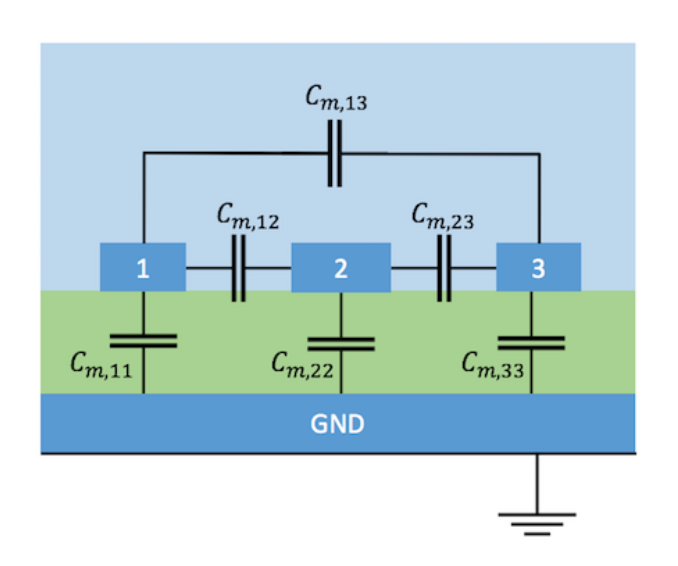
\includegraphics[width=\linewidth]{Figures/Electrodes/lumped_capacitance_scheme_better.png}
\end{minipage}
\begin{minipage}{0.38\textwidth}
	\begin{equation*}
	\Leftrightarrow
	\bm{C}^m = 
	\begin{pmatrix}
	C_{11}^m & C_{12}^m & C_{13}^m \\ 
	C_{21}^m & C_{22}^m & C_{23}^m \\
	C_{31}^m & C_{32}^m & C_{33}^m
	\end{pmatrix}
	\end{equation*}
\end{minipage}
\caption{Scheme representing an hypothetical electric modeling a system composed 3 electrodes $\{1,2,3\}$ surrounded by an electric ground $GND$. Each capacitance coupling corresponds to a term of the associated Mutual capacitance matrix. The diagonal terms $C_{ii}^m$ of the mutual capacitance matrix is called the self-capacitance and is modeled by a capacitance linking an electrode $i$ to the ground.}
\label{fig:lumped-capacitance}
\end{figure}

Each term $\bm{C}_{ij}^m$ can be interpreted as a lumped capacitance between two electrodes $i$ and $j$ and as such, are represented with the common parallel-plate capacitor symbol. One can note that the diagonal mutual capacitance terms $\bm{C}_{ii}^m$ are interpreted as the capacitance between the electrode $i$ and the ground (here the copper chassis). It is important to note that this matrix does not represent the relation between the electric charge $\vec{Q}$ and potential $\vec{V}$ of the electrodes of the system and therefore the equation \ref{eq:capacitance-definition-matrix} cannot be applied with the mutual capacitance matrix. Instead, the mutual capacitance matrix should be used as a modelization and interpretation tool. It is possible to obtain the Maxwell capacitance matrix from the mutual capacitance matrix according to:

\begin{equation} 
\label{eq:mutual-to-maxwell}
\bm{C} = 
\begin{pmatrix}
C_{11} & C_{12} & \cdots & C_{1N} \\ 
C_{21} & C_{22} & \cdots & C_{2N} \\ 
\vdots & \vdots & \ddots & \vdots \\ 
C_{N1} & C_{N2} & \cdots & C_{NN}
\end{pmatrix}
 = 
\begin{pmatrix}
\sum_{j=1}^N C_{1j}^m & -C_{12}^m & \cdots & -C_{1N}^m \\[0.3em]
-C_{21}^m & \sum_{j=1}^N C_{2j}^m & \cdots & -C_{2N}^m \\[0.3em]
\vdots & \vdots & \ddots & \vdots \\[0.3em] 
-C_{N1}^m & -C_{N2}^m & \cdots & \sum_{j=1}^N C_{Nj}^m
\end{pmatrix}
\end{equation}

With the interpretation of the mutual matrix as lumped capacitances, we see that the diagonal terms $\bm{C}_{ii}$ of the Maxwell capacitance matrix are simply the equivalent capacitance to all the lumped mutual capacitance $\bm{C}_{ij}$ put in parallel $C_{ii} = \sum_{j=1}^N C_{ij}^m$. As the non-diagonal terms of the Maxwell and the mutual capacitance matrix are opposite, the mutual capacitance matrix is also symmetric.

COMSOL offers a functionality called Stationary Source Sweep to evaluate the elastance and the capacitance matrices. Considering the equation \ref{eq:elastance-matrix}, a terminal $j$ is excited with an electric charge $Q_j$ with the charges of all the other terminals are set to $Q_i=0 , i\neq j$. The electrostatic system is numerically solved and the coefficient of potential can be deduced from the electric potential of the terminals $V_i$:
\begin{equation}
\bm{P_{ij}} = \frac{V_i}{Q_j}
\end{equation}
This procedure is repeated for each terminal until the full elastance matrix $\bm{P}$ is evaluated. Using the equations \ref{eq:maxwell-capacitance-matrix} and \ref{eq:mutual-to-maxwell}, the capacitance matrices can also be evaluated. In order to facilitate the discussion, the indexes of the matrices are swapped with the label of the electrodes. 

In the case of the Planar38 design, the correspondence between indexes and label is:
$$\{ top, bottom \} = \{A,B\} = \{ 1, 2\}$$
With the default parameters, the elastance and capacitance matrices are evaluated to:
\begin{equation} 
\label{eq:planar38-matrix-evaluation}
\begin{array}{rrccclc}
 & \bm{P} = &
 \begin{pmatrix}
P_{AA} & P_{AB} \\ 
P_{BA} & P_{BB}
\end{pmatrix}
&=&
\begin{pmatrix}
1.42 & 1.04 \\
1.04 & 1.42
\end{pmatrix}
& \cdot 10^{11} & [\textsf{F}^{-1}] \\
\Rightarrow & \bm{C} = &
\begin{pmatrix}
C_{AA} & C_{AB} \\ 
C_{BA} & C_{BB}
\end{pmatrix}
&=&
\begin{pmatrix}
14.92 & -10.86 \\
-10.86 & 14.92
\end{pmatrix}
& \cdot 10^{-12} & [\textsf{F}] \\
\Rightarrow & \bm{C}^m = &
\begin{pmatrix}
C_{AA}^m & C_{AB}^m \\ 
C_{BA}^m & C_{BB}^m
\end{pmatrix}
&=&
\begin{pmatrix}
4.06 & 10.86 \\
10.86 & 4.06
\end{pmatrix}
& \cdot 10^{-12} & [\textsf{F}]
\end{array}
\end{equation}
 
As expected from a similarly designed parallel-plate capacitor using the equation \ref{eq:capacitor-basic}, the Mutual capacitance are close the tens of picoFarad. As expected from the interpretation of the Mutual capacitance matrix, all of its terms are positive. Observing the Mutual capacitance matrix, we note that the capacitance between the electrodes $C_{AB}^m=10.86pF$ is greater than the self-capacitance of the electrodes $C_{AA}^m = C_{BB}^m = 4.06pF$. According to the parallel-plate capacitor equation \ref{eq:capacitor-basic}, there are multiple arguments pointing towards an opposite observation: the grounded chassis is surrounding the electrodes, presenting very large area and the distance electrode-chassis is smaller than the height of the crystal. However, the self-capacitance is mainly formed in the vacuum between the absorber and the chassis, with a relative electric permittivity $\epsilon_r(vaccum)=1$ whereas the mutual capacitance between the electrodes $A$ and $B$ is forming in the germanium crystal which imposes a relative permittivity of $\epsilon_r(Germanium)=16.3$. This  significant difference in material permittivity explains the hierarchy of the mutual capacitance for the Planar 38 design.

In the case of the FID38 design, the correspondence between indexes and labels is:
$$\{A,B,C,D\} = \{1,2,3,4\}$$
$$\{ Top Veto, Top Collect, Bottom Veto, Bottom Collect \} = \{A,B,C,D\} = \{ 1,2,3,4\}$$
With default parameters, the elastance and capacitance matrices are evaluated to:

\begin{equation} 
\label{eq:fid38-matrix-evaluation}
\begin{array}{rrccclc}
 & \bm{P} = &
 \begin{pmatrix}
P_{AA} & P_{AB} & P_{AC} & P_{AD} \\ 
P_{BA} & P_{BB} & P_{BC} & P_{BD} \\ 
P_{CA} & P_{CB} & P_{CC} & P_{CD} \\ 
P_{DA} & P_{DB} & P_{DC} & P_{DD}
\end{pmatrix}
&=&
\begin{pmatrix}
2.23 & 1.92 & 1.71 & 1.69 \\
1.92 & 2.34 & 1.69 & 1.68 \\
1.71 & 1.69 & 2.23 & 1.92 \\
1.69 & 1.68 & 1.92 & 2.34 \\
\end{pmatrix}
& \cdot 10^{11} & [\textsf{F}^{-1}] \\
\Rightarrow & \bm{C} = &
\begin{pmatrix}
C_{AA} & C_{AB} & C_{AC} & C_{AD} \\ 
C_{BA} & C_{BB} & C_{BC} & C_{BD} \\ 
C_{CA} & C_{CB} & C_{CC} & C_{CD} \\ 
C_{DA} & C_{DB} & C_{DC} & C_{DD}
\end{pmatrix}
&=&
\begin{pmatrix}
18.25 & -10.19 & -4.02 & -2.58 \\
-10.19 & 15.94 & -2.58 & -1.98 \\
-4.02 & -2.58 & 18.25 & -10.19 \\
-2.58 & -1.98 & -10.19 & 15.94 \\
\end{pmatrix}
& \cdot 10^{-12} & [\textsf{F}] \\
\Rightarrow & \bm{C}^m = &
\begin{pmatrix}
C_{AA}^m & C_{AB}^m & C_{AC}^m & C_{AD}^m \\ 
C_{BA}^m & C_{BB}^m & C_{BC}^m & C_{BD}^m \\ 
C_{CA}^m & C_{CB}^m & C_{CC}^m & C_{CD}^m \\ 
C_{DA}^m & C_{DB}^m & C_{DC}^m & C_{DD}^m
\end{pmatrix}
&=&
\begin{pmatrix}
1.46 & 10.19 & 4.02 & 2.58 \\
10.19 & 1.18 & 2.58 & 1.98 \\
4.02 & 2.58 & 1.46 & 10.19 \\
2.58 & 1.98 & 10.19 & 1.18 \\
\end{pmatrix}
& \cdot 10^{-12} & [\textsf{F}]
\end{array}
\end{equation}

The observations made previously for the Planar38 design still holds for the FID38 design: capacitances are close to tens of picoFarad and the self-capacitance term are dominated. In particular, we note that the Mutual capacitance is dominated by the terms $C_{AB}^m=C_{BA}^m=C_{CD}^m=C_{DC}^m=10.19pF$. Indeed, as the electrodes $A,B$ and $C,D$ are interleaved, their capacitive coupling is high as it emulates a situation with two close plates. The next higher term is $C_{AC}^m=4.02pF$ coming from the two veto electrodes which are facing each other and coming very close to one another near the equator leading to an increase in coupling. The hierarchy of the remaining term can be explained by the fact that their are more veto electrode rings than collect electrode rings, thus emulating a higher electrode area in the equation \ref{eq:capacitor-basic}.

\subsection{Sensitivity Calculation}
\label{par:sensitivity-calculation}

In the case of the FID38, we try to model the generation of the ionization signal. We consider an ideal detector with default parameters (A,B,C,D = -1,+4,+1,-4 V) with no trapping and a single electron-hole pair created at a desired location. We assume that the electric charges will drift following exactly the electric field lines. The disposition of the electrodes for the FID38 design illustrated in the scheme \ref{fig:fid38-scheme} mentions four possible locations for the recoils to happen. Each location will have charges drifting towards a specific combination of electrodes inducing an electric charge perturbation $\vec{Q}$ according to the integration of the Shockley-Ramo theorem \ref{eq:ramo-theorem-integrated}. The electric potential signal $\vec{V}$ created by the electric charge perturbation $\vec{Q}$ with the application of the equation \ref{eq:capacitance-definition-matrix} along with the evaluation of the Maxwell capacitance matrix \ref{eq:fid38-matrix-evaluation}. The electric charge perturbation is assumed to be created by a 1keV electronic recoil, creating a number $N_p = 1000/3 = 333$ of electron-hole pairs.
In the case of the Planar38, we refer to the equation \ref{eq:plana38-induced-charges} for the electric charge perturbation vector. The voltage signal vector is thus:

\begin{equation}
\label{eq:planar38-sensitivity}
\vec{V}_{event} = \bm{P} \vec{Q}_{event} =
\begin{bmatrix}
- P_{AA} + P_{AB} \\ - P_{BA} + P_{BB}
\end{bmatrix}
\cdot N_p \cdot e
= 
\begin{bmatrix}
-0.39 \\  \\ 0.39
\end{bmatrix}
\cdot N_p \cdot e \cdot 10^{11}
= 
\begin{bmatrix}
-2.08 \\ 2.08 
\end{bmatrix}
[\mu V/keV]
\end{equation}

In the case of the FID38, we refer to the equation \ref{eq:fid38-induced-charges} for the four possible electric charges perturbation vector. There are four corresponding voltage signal vectors:

\begin{align}
\label{eq:fid38-sensitivity}
\vec{V}_{bulk} = \bm{P} \vec{Q}_{bulk} &=
\begin{bmatrix}
- P_{AB} + P_{AD} \\
- P_{BB} + P_{BD} \\
- P_{CB} + P_{CD} \\
- P_{DB} + P_{DD} \\
\end{bmatrix}
\cdot N_p \cdot e
= 
\begin{bmatrix}
-0.23 \\ -0.66 \\ 0.23 \\ 0.66
\end{bmatrix}
\cdot N_p \cdot e \cdot 10^{11}
=
\begin{bmatrix}
-1.23 \\ -3.52 \\ 1.23 \\ 3.52
\end{bmatrix}
[\mu V/ keV]
\\
\vec{V}_{veto, top} = \bm{P} \vec{Q}_{veto,top} &=
\begin{bmatrix}
+ P_{AA} - P_{AB} \\
+ P_{BA} - P_{BB} \\
+ P_{CA} - P_{CB} \\
+ P_{DA} - P_{DB} \\
\end{bmatrix}
\cdot N_p \cdot e
= 
\begin{bmatrix}
0.31 \\ -0.42 \\ 0.02 \\ 0.01
\end{bmatrix}
\cdot N_p \cdot e \cdot 10^{11}
= 
\begin{bmatrix}
1.65 \\ -2.24 \\ 0.11 \\ 0.05
\end{bmatrix}
[\mu V/keV]
\\
\vec{V}_{veto,bottom} = \bm{P} \vec{Q}_{veto,bottom} &=
\begin{bmatrix}
- P_{AC} + P_{AD} \\
- P_{BC} + P_{BD} \\
- P_{CC} + P_{CD} \\
- P_{DC} + P_{DD} \\
\end{bmatrix}
\cdot N_p \cdot e
= 
\begin{bmatrix}
0.02 \\ 0.01 \\ -0.31 \\ -0.42
\end{bmatrix}
\cdot N_p \cdot e \cdot 10^{11}
= 
\begin{bmatrix}
0.11 \\ 0.05 \\ -1.65 \\ 2.24
\end{bmatrix}
[\mu V/keV]
\\
\vec{V}_{equator} = \bm{P} \vec{Q}_{equator} &=
\begin{bmatrix}
- P_{AA} + P_{AC} \\
- P_{BA} + P_{BC} \\
- P_{CA} + P_{CC} \\
- P_{DA} + P_{DC} \\
\end{bmatrix}
\cdot N_p \cdot e
= 
\begin{bmatrix}
0.52 \\ 0.23 \\ -0.52 \\ -0.23
\end{bmatrix}
\cdot N_p \cdot e \cdot 10^{11}
= 
\begin{bmatrix}
2.77 \\ 1.23 \\ -2.77 \\ -1.23
\end{bmatrix}
[\mu V/keV]
\end{align}

The first thing one can note is that even though for each case the electron and hole were collected by two electrode, an electric potential perturbation was created on all the electrodes. This phenomenon is referred as "capacitive cross-talk". Then, we note that the amplitude of the signal, referred as "electrode sensitivity" $S_{type}^{A} = |\vec{v}/e|$ is not equal among the collecting electrodes comparing different events. We can quantify this cross-talk by calculating the ratio $X_{type}$ between the signal induced on a non-collecting electrode over the signal induced on a collecting electrode:

The sensitivity of an electrode corresponds to the amplitude of the voltage signal weighted by the input energy and is expressed in $\mu V/keV$. Considering the results of the equation \ref{eq:planar38-sensitivity} and \ref{eq:fid38-sensitivity}, for an electrode $X$ and a kind of event $type$, the sensitivity is expressed as:

\begin{equation}
S_{X, type} = | V_{X,type} | \quad \textsf{in} \quad [\mu V/keV]
\end{equation}

We can compare the FID38 design "efficiency" by comparing the Maxwell capacitance matrix, obtained in equations \ref{eq:planar38-matrix-evaluation} and \ref{eq:fid38-matrix-evaluation}, to a reference ideal two plate capacitance $C_{ref}(type, A)$ of the same sensitivity that the considered recoil $type$ and electrode $A$. This reference capacitance is composed of a ground and a unique terminal such that the charge perturbation is $q_{ref}=-e$ and the induced electric potential $v_{ref}(type)$ is expressed as:

\begin{equation}
C_{X,type}^{ref} = \left( \frac{S_{X,type}}{N_p \cdot e} \right)^{-1}
\end{equation}

In the case of the Planar38 detector, there is only one type of event for two electrodes with equal sensitivities. The reference capacitance is expressed as:

\begin{equation}
\label{eq:planar38-reference-capacitance}
C_{top}^{ref}
= C_{bottom}^{ref}
= \left( | -P_{AA} + P_{AB} |\right)^{-1}
= \left( | -P_{AB} + P_{BB} |\right)^{-1}
= 0.39 \cdot 10^{11}
= 26 \cdot 10^{-12} [F]
\end{equation}

The equivalent reference capacitance is 26 pF. It is greater than any term of the capacitance matrices for the Planar38, which indicates that this design as worse efficiency than the two-plate capacitor design. The calculation of the sensitivity in equation \ref{eq:planar38-sensitivity} and the reference capacitance in equation \ref{eq:planar38-reference-capacitance} shows that the sensitivity is proportional to the term $| -P_{AA} + P_{AB} | = | -P_{AB} + P_{BB} |$. This term can be interpreted as the difference between the diagonal terms, $P_{AA}$ and $P_{BB}$, of the elastance matrix and the non-diagonal term $P_{AB}$ expressing the coupling between the two collecting electrodes (here $A$ and $B$). (Should be discussed with the fid38, this structure is confirmed there).

In the case of the FID38 detector, there are four types of events and four electrodes, resulting to a total of 16 sensitivities as seen in equation \ref{eq:fid38-sensitivity}. Among all this values, some are more relevant to the ionization channel operation than the others.

The auxiliary electrodes $A,C$ are as veto and their signal is used to determine if an event is a bulk or veto event (see fiducial cut in Chapter Neutron). Therefore, the sensitivities of these veto electrodes are relevant in the case of $veto$, $S_{A, veto}=S_{C, veto}$, and $equator$ recoils, $S_{A, equator}=S_{C, equator}$. The main electrodes $B,D$ are used to reconstruct the ionization energy of the $bulk$ events. Thus, their sensitivities are relevant for $bulk$ recoils, $S_{B, bulk}=S_{D, bulk}$. From these sensitivities, the equivalent reference capacitances are deduced:

\begin{align}
C_{A, veto}^{ref} = C_{C, veto}^{ref}
= \left( | P_{AA} - P_{AB} |\right)^{-1}
= \left( | -P_{CC} + P_{CB} |\right)^{-1}
= 0.31 \cdot 10^{11}
&= 32 \cdot 10^{-12} [F]
\\
C_{A, equator}^{ref} = C_{C, equator}^{ref}
= \left( | P_{AA} - P_{AC} |\right)^{-1}
= \left( | -P_{CC} + P_{AC} |\right)^{-1}
= 0.52 \cdot 10^{11}
&= 19 \cdot 10^{-12} [F]
\\
C_{B, bulk}^{ref} = C_{D, bulk}^{ref}
= \left( | -P_{BB} + P_{BD} |\right)^{-1}
= \left( | P_{DD} - P_{BD} |\right)^{-1}
= 0.66 \cdot 10^{11}
&= 15 \cdot 10^{-12} [F]
\end{align}

There is a specific cross-talk and sensitivity for each type of events. When analyzing the detector data, there should therefore be a specific calibration and cross-talk correction associated to each of this type of signal.
However, to this day, the EDELWEISS and R\&D experiments have only use a single analysis pipeline with a single calibration value for each electrodes and a single cross-talk correction matrix, independently of the type of event. Furthermore, the analysis seemed valid and no significant deviation was observed from the simple, yet wrong, ionization model where events creating the same amounts of electron-hole pairs presents the same electrode sensitivity and capacitive cross-talk. This can be explained by the fact that the capacitances of the detector are dominated by the greater capacitance of the cabling. It is important to recall that this work is focused on the capacitance of the electrodes of a detector, and did not considered the capacitance of the cabling between the electrodes and the amplifying electronics. In the experimental setup, the electrodes are cabled to the electronics with coaxial cables. While a coaxial cable shield the signal from the exterior interferences, it also create a significant capacitive coupling between the ground and the core (in this case, the electrode). Let's assume a of $50$pF capacitance between the ground and each electrodes, the elastance matrix is now evaluated to:

\begin{equation}
\bm{C}^{cabling} = \bm{C} + \mathbb{1} \cdot 50 \cdot 10^{-12} [\textsf{F}]
\quad \Rightarrow \quad
\bm{P}^{cabling} = 
\begin{bmatrix}
  0.151 & 0.024 & 0.011 & 0.008\\
  0.024 & 0.156 & 0.008 & 0.007\\
  0.011 & 0.008 & 0.151 & 0.024\\
  0.008 & 0.007 & 0.024 & 0.156\\
\end{bmatrix}
\cdot 10^{11}
\end{equation}

\begin{equation}
\bm{P}_{PL38}^{cabling}
=
\begin{bmatrix}
  0.158 & 0.027 \\
  0.027 & 0.158 \\
\end{bmatrix}
\cdot
10^{11}
\end{equation}

In the case of the Planar38 with the capacitive cabling:

\begin{equation}
\vec{V}_{event}
=
\begin{bmatrix}
0.131 \\
-0.131
\end{bmatrix}
\cdot 10^{11}
=
\begin{bmatrix}
0.71 \\
-0.71
\end{bmatrix}
[\mu V/keV]
\end{equation}

\begin{equation}
C_{top, bottom}^{ref}
= 0.131 \cdot 10^{11}
= 76 \cdot 10^{-12} [F]
\end{equation}

In the case of the FID38 with the capacitive cabling:

\begin{align}
\vec{V}_{bulk}
=
\begin{bmatrix}
  -0.016 \\ -0.149 \\ 0.016 \\ 0.149\\
\end{bmatrix}
\cdot 10^{11}
= &
\begin{bmatrix}
-0.05 \\ -0.80 \\ 0.05 \\ 0.80
\end{bmatrix}
[\mu V/keV]
\\
\vec{V}_{veto,top}
=
\begin{bmatrix}
  0.127 \\ -0.132 \\ 0.003 \\ 0.001\\
\end{bmatrix}
\cdot 10^{11}
= &
\begin{bmatrix}
0.69 \\ -0.75 \\ 0 \\ 0
\end{bmatrix}
[\mu V/keV]
\\
\vec{V}_{veto,bottom}
=
\begin{bmatrix}
  -0.003 \\ -0.001 \\ -0.127 \\ 0.132\\
\end{bmatrix}
\cdot 10^{11}
= &
\begin{bmatrix}
0 \\ 0 \\ -0.69 \\ 0.75
\end{bmatrix}
[\mu V/keV]
\\
\vec{V}_{equator}
=
\begin{bmatrix}
  0.140 \\ 0.016 \\ -0.140 \\ -0.016\\
\end{bmatrix}
\cdot 10^{11}
= &
\begin{bmatrix}
0.75 \\ 0.05 \\ -0.75 \\ -0.05
\end{bmatrix}
[\mu V/keV]
\end{align}


\begin{align}
C_{A, veto}^{ref} = C_{C, veto}^{ref}
= 0.127 \cdot 10^{11}
&= 78.7 \cdot 10^{-12} [F]
\\
C_{A, equator}^{ref} = C_{C, equator}^{ref}
= 0.140 \cdot 10^{11}
&= 71.4 \cdot 10^{-12} [F]
\\
C_{B, bulk}^{ref} = C_{D, bulk}^{ref}
= 0.149 \cdot 10^{11}
&= 67.1 \cdot 10^{-12} [F]
\end{align}

We see that by adding the capacitance of the cabling, the cross-talk phenomenon is significantly lessened and that the electrode sensitivities are very close to 0.14 in absolute value for all the types of events. The small variation of cross-talk and sensitivities were surely "absorbed" in the resolution of the ionization channel in the previous EDELWEISS and IP2I R\&D analysis, leading to an overall very correct result. As a complement, let's add that as the capacitive coupling with the ground through the coaxial cabling is increased, the cross-talk and difference in sensitivity vanish. In the case of EDELWEISS-III with a cabling of capacitance $>100$pF, the simple ionization signal generation model holds.

In order to fully appreciate the impact of the cabling capacity, the figure \ref{fig:predict-corner-plot} presents the corner plot of the simulation of 1000 events of each recoil type in a FID38 detector with (black points) and without (colored points) 50pF cabling capacitance. Each event is associated to a voltage signal vector $\vec{V}$. Each term is plotted on the corner plot similarly to the analysis of real events. The events were simulated with a normal distribution centered on the sensitivities calculated in equation \ref{eq:fid38-sensitivity} and with a standard deviation of $1\mu V/keV$.

\begin{figure}
\centering
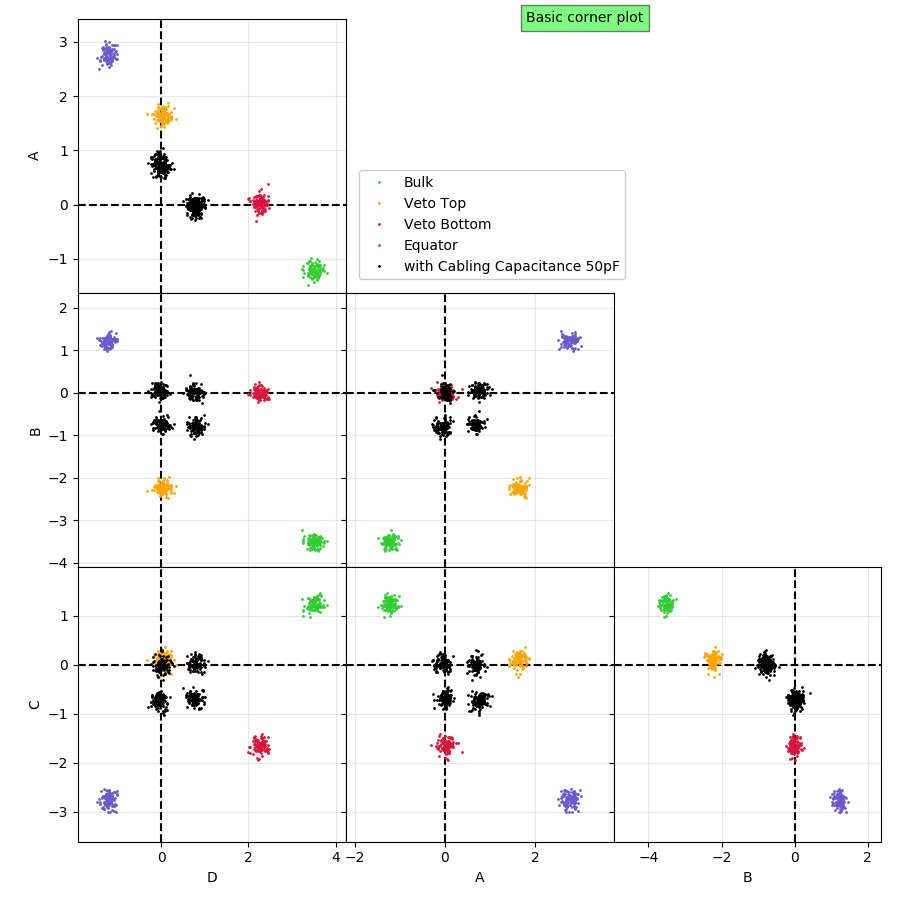
\includegraphics[width=\linewidth]{Figures/Electrodes/predict_corner_plot.png}
\caption{Simulation of the expected signal with a FID38 detector with cabling (black circles) and without capacitive cabling (color squares). There are 1000 points for each event types, and each channel is modeled by a gaussian distribution of variance 100eV.}
\label{fig:predict-corner-plot}
\end{figure}

With the 50pF cabling capacitance, the 4 recoil type form the usual "square" pattern similar to what is obtained in the next Chapter \ref{ChapterNeutron} discussing analysis of the neutron run with RED80. The square pattern emerges from the low cross-talks of about $0.05/0.80=6\%$ and $0.05/0.75=7\%$.

Without any cabling capacitance, the recoil types are more distant from the origin, which illustrates the greater sensitivities in this case. The 4 recoil populations do not form a square pattern anymore and presents the high cross-talk obtained in the previous equations, $1.23/3.52=35\%$ and $1.23/2.77=44\%$.


\subsection{Noise and Resolution Calculation}
\label{par:ion-resolution-calculation}

The previous paragraph presented how, with low cabling capacitance, the capacitive coupling between each electrodes affects the sensitivity of the ionization channel. This paragraph discusses the impact of this capacitive coupling on the noise affecting the measurement and eventually the resolution of the ionization channel.

A previous paragraph \ref{par:electronics-ionization} already presented the noise propagation and resolution calculation for the future HEMT electronics. These calculations were based on a single HEMT line cabled on a single capacitance $C_d$ representing an electrode of the detector. We will now study how the noise calculation is affected by the coupling of multiple HEMT lines.

In order to motivate this study, the noise calculation is first done on a very simple model: the Planar38 design with a heavily simplified HEMT line featuring only the polarization resistor and its associated Johnson noise. The scheme of this simplified model is presented in the figure \ref{fig:scheme-planar38-simplified}. Thanks to the superposition theorem and Thevenin-Norton transformations of the electric circuit, it is possible to propagate the two Johnson noise source $e_{J,A}$ and $e_{J,B}$ to the measurement point $S_B$. The total noise and its components measured at $S_B$ are plotted as functions of the frequency on the left figure \ref{fig:planar38-analytical-results}. Event though the original Johnson voltage noise source are modeled as white noise whose levels are independent from the frequency, the total voltage noise affecting the measurement at node $S_B$ presents a low-pass filter profile. This is consistent with the studied electric system as the node $S_B$ is linked to the electric ground through the two capacitors $C_{22}$ and $C_{11}$: at high frequency, the electric potential of the node $S_B$ tends be null. The dominant component of the noise is the Johnson noise $e_{J,B}$ of the Hemt line of the electrode $B$ where the measurement is made. It is less dampened than the other Johnson noise source $e_{J,A}$ which is filtered by the capacitance $C_{12}$ coupling the two electrodes $A$ and $B$. The right figure \ref{fig:planar38-analytical-results} shows the ratio of the two Johnson noise components $e_{J,A}/e_{J,B}$ as a function of the frequency.

\begin{figure}
\centering
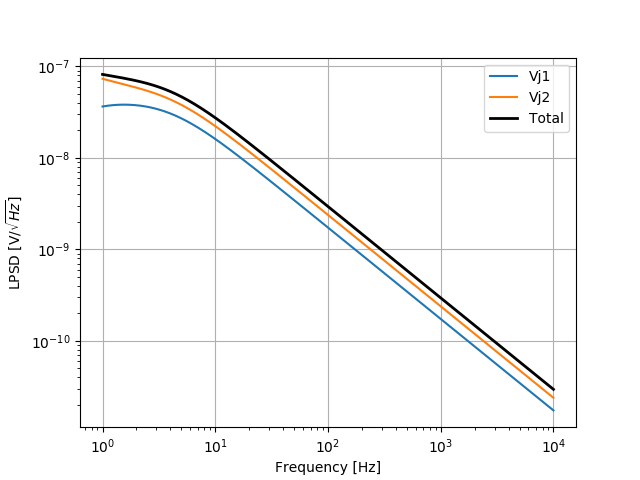
\includegraphics[width=0.48\textwidth]{Figures/Electrodes/planar38_johnson_propagation.png}
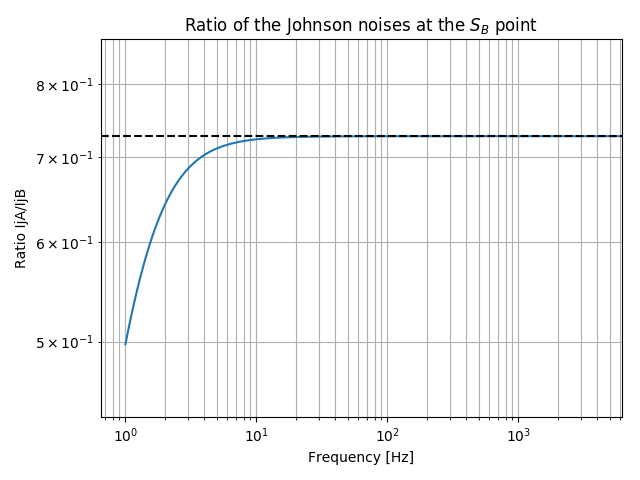
\includegraphics[width=0.48\textwidth]{Figures/Electrodes/planar38_comparison_johnson.png}
\caption{
\textbf{Left:} Total voltage noise measured at the node $S_B$ along with its components as functions pf the frequency.
\textbf{Right:} Ratio of two Johnson noise components at the node $S_B$ as a function of the frequency.
}
\label{fig:planar38-analytical-results}
\end{figure}

This ratio is consistent with a high-pass filtering assured by the coupling capacitance $C_{12}$. Analytically, the ratio is expressed as:

\begin{equation}
\label{eq:planar38_analytical}
\frac{e_{J,A}(S_B)}{e_{J,B}(S_B)}
=
  \frac{ j \omega R_{polar} C_{12}^m }{ 1 + j \omega R_{polar} \left( C_{12}^m + C_{11}^m \right) } \
\xrightarrow[{f\to \infty}]{}
  \frac{ C_{12}^m }{ C_{12}^m + C_{11}^m }
=
  \frac{ -C_{12} }{ C_{11} }
=
  \frac{ 10.86 \cdot 10^{-12} }{ 14.92 \cdot 10^{-12} }
\approx
  0.73
\end{equation}

Above the cutoff frequency of about $3.3$Hz, the ratio tends to $0.73$. According to the previous equation \ref{eq:planar38_analytical}, the ratio depends on the ratio of the non-diagonal over the diagonal terms of the Maxwell capacitance matrix of the Planar38 detector (from equation \ref{eq:planar38-matrix-evaluation}). This ratio of Maxwell capacitance is comprised between 0 and 1, and reaches its maximum if the capacitive coupling $C_{12}^m$ between the two electrodes $A$ and $B$ is much greater than the self-capacitance $C_{11}^m$ of the electrode $A$.

As the two Johnson noise are not correlated, their squared noise level is added to form the total noise level which is tends to be $\sqrt{1^2 + (0.73)^2} = 1.24$ times the original Johnson noise level caused by $e_{J,B}$. With the given Planar38 design with the simplified HEMT line, the noise level is increased by $24\%$ from approximately $10$Hz. The effect of the coupling between the electrodes is far from negligible and should be properly studied for the two reference design FID38 and Planar38 with a full Hemt line model.

\begin{landscape}
\begin{figure}
\centering
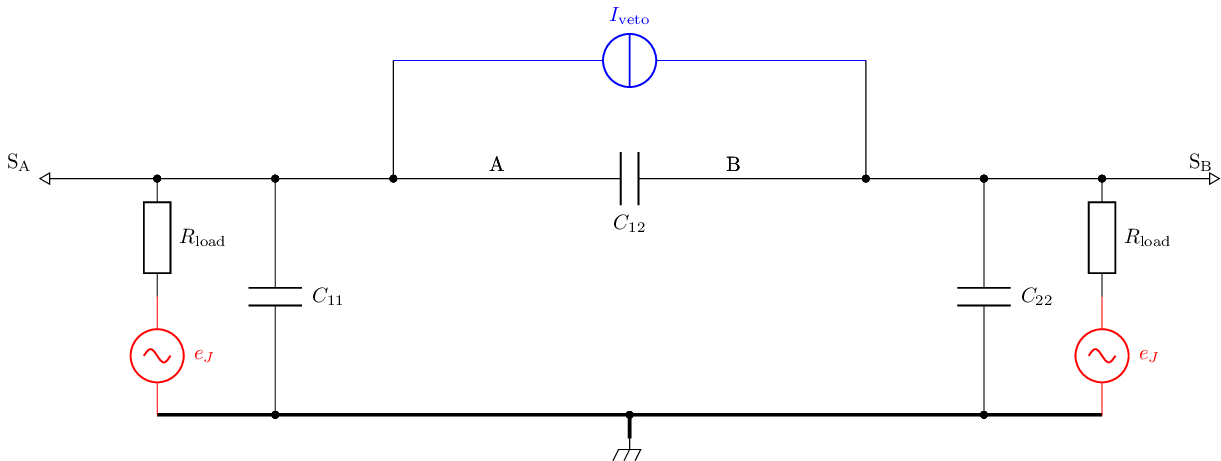
\includegraphics[height=0.25\textheight, width=\linewidth, keepaspectratio]{Figures/Electrodes/scheme_planar38_analytical.png}
\caption{Electric scheme of the FID38 with a hemt line for each electrode. The lumped capacitance model is used to represent the capacities of the electrodes. Thus, the scheme uses the term of the mutual capacitance matrix. REDO WITH BETTER FONT SIZE}
\label{fig:scheme-planar38-simplified}
\end{figure}

\begin{figure}
\centering
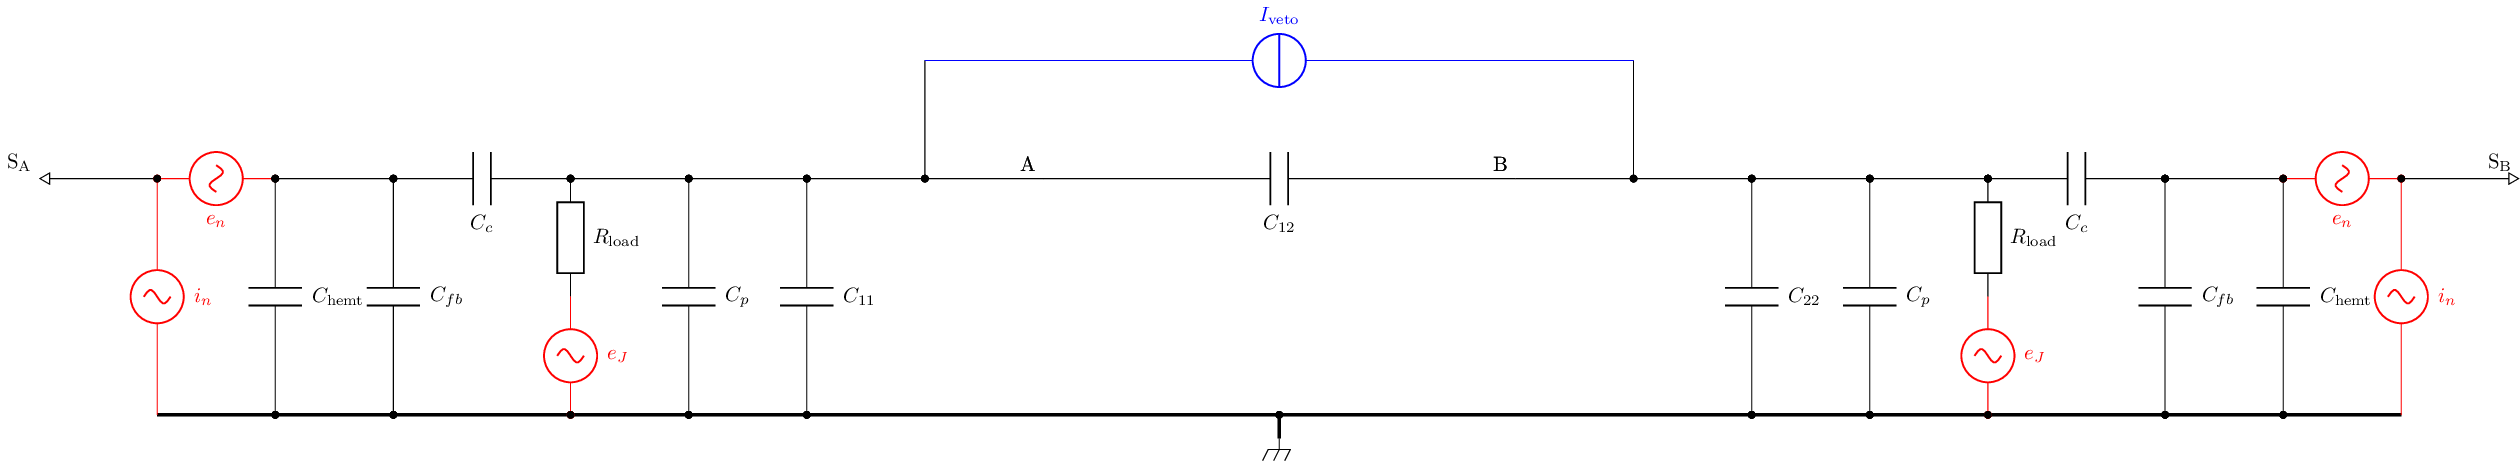
\includegraphics[height=0.25\textheight, width=\linewidth, keepaspectratio]{Figures/Electrodes/scheme_planar38.png}
\caption{Electric scheme of the Planar38 with a hemt line for each electrode. The lumped capacitance model is used to represent the capacities of the electrodes. Thus, the scheme uses the term of the mutual capacitance matrix. REDO WITH BETTER FONT SIZE}
\label{fig:scheme-planar38-full}
\end{figure}
\end{landscape}

The Planar38 detector cabled with the full Hemt line is illustrated in the scheme \ref{fig:scheme-planar38-full}. The detector is composed of the three mutual capacitance $C_{ij}^m$ linked to the nodes $A,B$. There is a measurement node for each electrode $S_A$ and $S_B$, acting as an ideal voltmeter with the electric ground as reference. There is a total of 6 noise sources coming from the Hemt lines. The signal induced by an event is modeled as a transient current source $I_{event}=N_p \cdot e \cdot \delta(t)$ between $A$ and $B$. The multiple noise source and the event signal are propagated to the measurement node $S_B$ using the numerical circuit resolution (see Lcapy module for Python).
% Noise propagation plot
The left figure \ref{fig:planar38-propagation} presents the total noise and its components measured at $S_B$ as a function of the frequency. The predominant noise are the Johnson noise $e_{J,B}$ of the Hemt line of the electrode $B$ at low frequency and the intrinsic current noise $i_{n,B}$ at high frequency. The Johnson noise $e_{J,A}$ from the other Hemt line of the electrode $A$ is slightly present below 2Hz, but is quickly dominated by the intrinsic voltage source $e_{n,B}$. In the end, we observe that the noise sources from the auxiliary HEMT line are heavily filtered and does not propagate significantly to the measurement node $S_B$. When comparing to the previous simplified electric circuit where the propagation was significant, one of the main difference is now the presence of the feedback capacitance, the hemt intrinsic capacitance and the cabling capacitance (Representing in this case 5+3+5 = 13pF). These capacitances are added to the diagonal term of the Maxwell capacitance matrix and reduce the propagation of the noise source through the coupling capacitance $C_{12}^m$.
% Noise vs Signal
The top right figure \ref{fig:planar38-propagation} presents the total noise power spectral density compared to the power spectrum of the signal induced by an event. Their shape are quite similar to a $1/f$ profile. From this functions, the Noise Equivalent Power is calculated and represented in the bottom right figure \ref{fig:planar38-propagation}. The NEP is an increasing function, therefore the majority of the information on the signal is associated to the low frequency. When integrating between 1Hz and infinity, the resolution is evaluated to $\sigma_B=34$eV. (bad? Can be compared to the initial simple model with a single Hemt and single electrode equivalent to the detector).

\begin{figure}
\centering
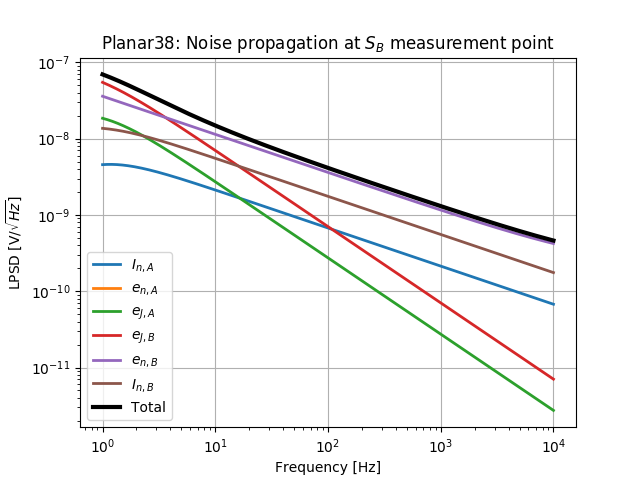
\includegraphics[width=0.48\textwidth]{Figures/Electrodes/planar38_noise_propagation.png}
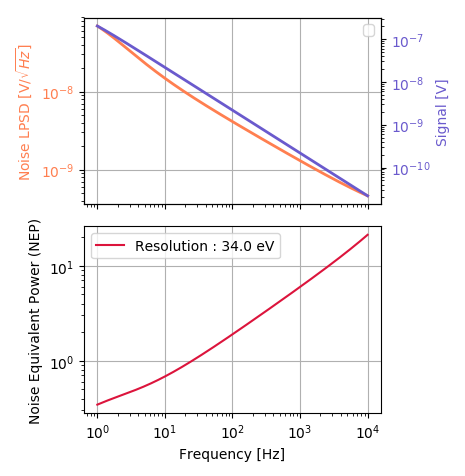
\includegraphics[width=0.48\textwidth]{Figures/Electrodes/planar38_nep_resolution.png}
\caption{
\textbf{Left:} Total voltage noise measured at the node $S_B$ along with its components as functions pf the frequency.
\textbf{Right:} Noise Power Spectral Density compared to Signal Power Spectrum, and Noise Equivalent Power with a Resolution of $\sigma_{B} = 34$eV.
}
\label{fig:planar38-propagation}
\end{figure}

% FID38 noise propagation
The FID38 detector cabled with the full Hemt line is illustrated in the scheme \ref{fig:scheme-planar38-full}. The detector is composed of the ten mutual capacitance $C_{ij}^m$ linked to the nodes $A,B,C,D$. There is a measurement node for each electrode $S_A, S_B, S_c, S_D$, acting as an ideal voltmeter with the electric ground as reference. There is a total of $4\times3=12$ noise sources coming from the four Hemt lines. Signals induced by events are modeled as transient current sources $I_{event}=N_p \cdot e \cdot \delta(t)$ between two electrode nodes depending on the considered recoil type. The multiple noise source and the event signals are propagated to the measurement node $S_B$ using the numerical circuit resolution (see Lcapy module for Python).
% Noise propagation plot
The left figure \ref{fig:planar38-propagation} presents the total noise and its components measured at $S_B$ as a function of the frequency. The predominant noise are the Johnson noise $e_{J,B}$ of the Hemt line of the electrode $B$ at low frequency and the intrinsic current noise $i_{n,B}$ at high frequency. The Johnson noise $e_{J,A}$ from the other Hemt line of the electrode $A$ is slightly present below 2Hz, but is quickly dominated by the intrinsic voltage source $e_{n,B}$. All in all, the results are quite similar to what was observed with the Planar38 design: the Johnson noise from the most coupled electrode is significant at very low frequency and is quickly dominated by the intrinsic voltage noise source of the Hemt line $B$. Again, this can be explained by a boosted diagonal term in the Maxwell capacitance matrix which heavily filter the noise sources from spreading to other Hemt line efficiently.
% Noise vs Signal
The top right figure \ref{fig:planar38-propagation} presents the total noise power spectral density compared to the power spectrum of the signal induced by the different recoil types of 1keV. Just as what was calculated in the equation \ref{eq:fid38-sensitivity} and discussed in the associated paragraph, the main sensitivity to take into account are $A,C$ for veto and equatorial event, and $B,D$ for the bulk events. The shapes of the noise and signals are quite similar to a $1/f$ profile. From this functions, the Noise Equivalent Power is calculated and represented in the bottom right figure \ref{fig:planar38-propagation}. The NEP is an increasing function, therefore the majority of the information on the signal is associated to the low frequency. When integrating between 1Hz and infinity, the resolution is evaluated to $\sigma_B=\sigma_D=28$eV and $\sigma_A=\sigma_C=32$eV. (bad? Can be compared to the initial simple model with a single Hemt and single electrode equivalent to the detector).

\begin{figure}
\centering
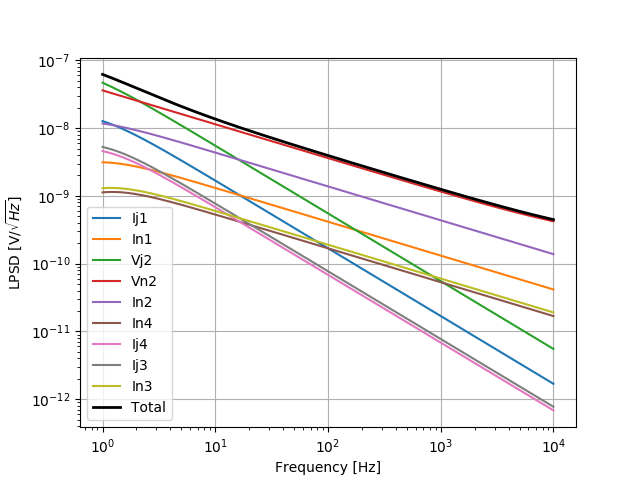
\includegraphics[width=0.48\textwidth]{Figures/Electrodes/fid38_noise_propagation.png}
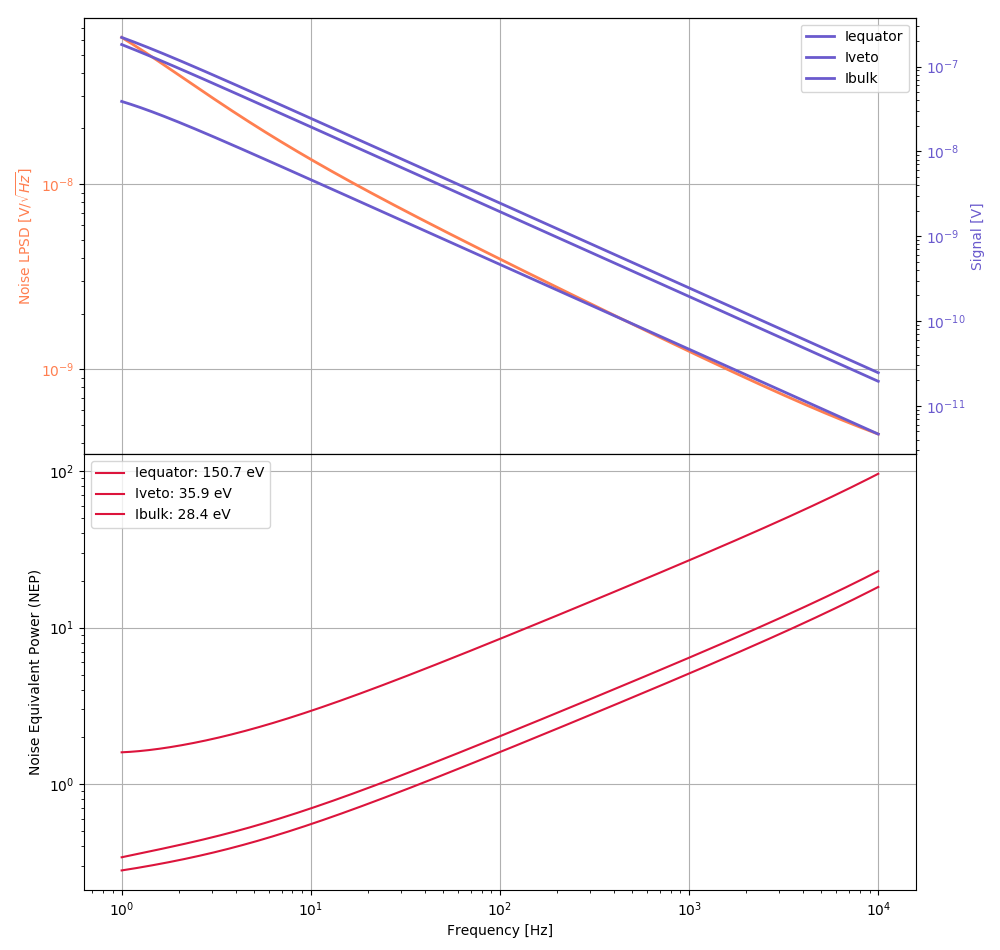
\includegraphics[width=0.48\textwidth]{Figures/Electrodes/fid38_nep_resolution.png}
\caption{
\textbf{Left:} Total voltage noise measured at the node $S_B$ along with its components as functions pf the frequency.
\textbf{Right:} Noise Power Spectral Density compared to Signal Power Spectrum, and Noise Equivalent Power with a Resolution of $\sigma_{B} = 28$eV.
}
\label{fig:fid38-propagation}
\end{figure}

% Planar38 Scan
The performance of a detector is partly quantified by the resolution of its ionization channel. Thus, the resolutions calculated previously for the Planar38 and FID38 are figure of merits. However, these calculation are long as they necessitate to simulate a detector design into COMSOL to calculate the Mutual capacitance matrix and then simulate the detector cabled with the hemt lines with Lcapy.

The resolution of the electrodes of a detector design depends on the whole Maxwell capacitance matrix (3 independent terms for the Planar38, and 10 independents terms for the FID38). It might be possible to access some basic trends by scanning over basic parameters.

The left figure \ref{fig:planar38-scan} is a graph of the calculated resolution as a function of the equivalent capacitance of the HEMT lines (cabling capacitance + feedback capacitance + intrinsic hemt capacitance). The capacitance of the Hemt line are appearing on the diagonal term of the Maxwell capacitance. Therefore, this parameter scan can be interpreted as studying the resolution as a function of the diagonal terms of the Maxwell capacitance terms.
Apart from the first point at very low capacitance, we observe that a high cabling capacitance increases the resolution of the ionization channels.

%{\color{blue} (More points ? Clear legend with a scanning on each elements (cabling, fb, hemt) ? Do it for fid38 also ?)}

The right figure \ref{fig:planar38-scan} is a graph of the resolution as a function of a global multiplier factor of the Maxwell capacitance matrix for the Planar38 design. A multiplier factor of 1 corresponds to a resolution calculation with the presented capacitance matrices presented in the equation \ref{eq:planar38-matrix-evaluation}. It is possible to artificially change all the capacitance terms of the capacitance matrix with this global multiplier factor. Compared to the previous scan on the diagonal term of the Maxwell matrix, this scan impact the whole matrix. In order to realistically apply this transformation, we could think of a up/down scaling of the detector size (increasing/reducing the area of the electrodes) or changing the electric permittivity with another absorber material. We observe that the resolution is almost proportional to the global multiplier factor.

These two observations are consistent with what could be expected from the very basic understanding of the ionization channel presented in the paragraph \ref{par:basic-ion-channel}: the resolution decreases as the capacitances of the detector decrease. 
In order to optimize the ionization channel, the research should be focused on lowering the capacitance of the cabling, and lowering the capacitances of the electrodes.
The cabling links the electrodes evaporated on the germanium crystal and the HEMT electronics. Its capacitance depends on the type of cabling (shielded, material) and is proportional to its length. As a result, lowering the cabling capacitance is ultimately a geometric challenge on the cryostat configuration and the suspended tower. Currently, the cabling capacitance is guaranteed to be lower than 20pF, and with should be expected to reach 5pF with further research.
The capacitance of the electrodes depends on the design of the detector and is heavily discussed in the next paragraph of this section.

\begin{figure}
\centering
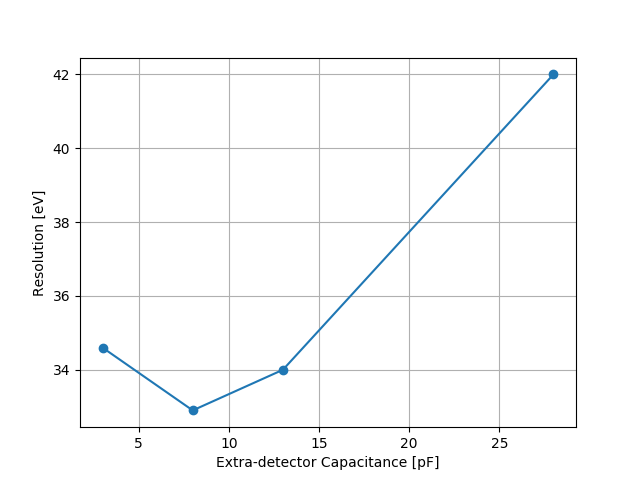
\includegraphics[width=0.48\textwidth]{Figures/Electrodes/scan_capacitance.png}
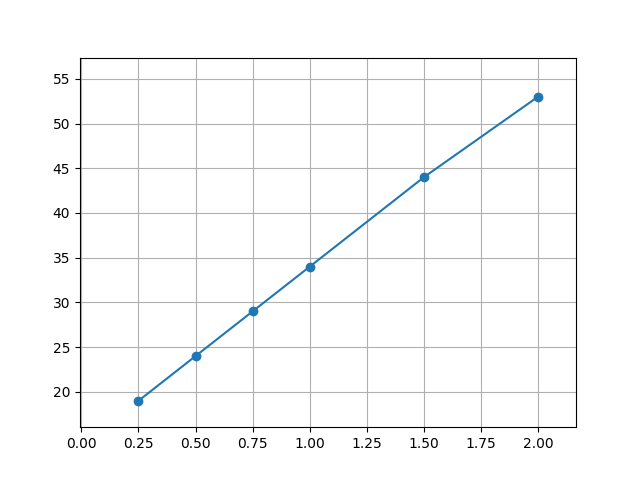
\includegraphics[width=0.48\textwidth]{Figures/Electrodes/scan_alpha.png}
\caption{
\textbf{Left:} Resolution of electrode B as a function of the extra-detector capacitance.
\textbf{Right:} Resolution of the electrode B as a function of a multiplicative factor of the Maxwell capacitance matrix.
}
\label{fig:planar38-scan}
\end{figure}



\begin{landscape}

\begin{figure}
\centering
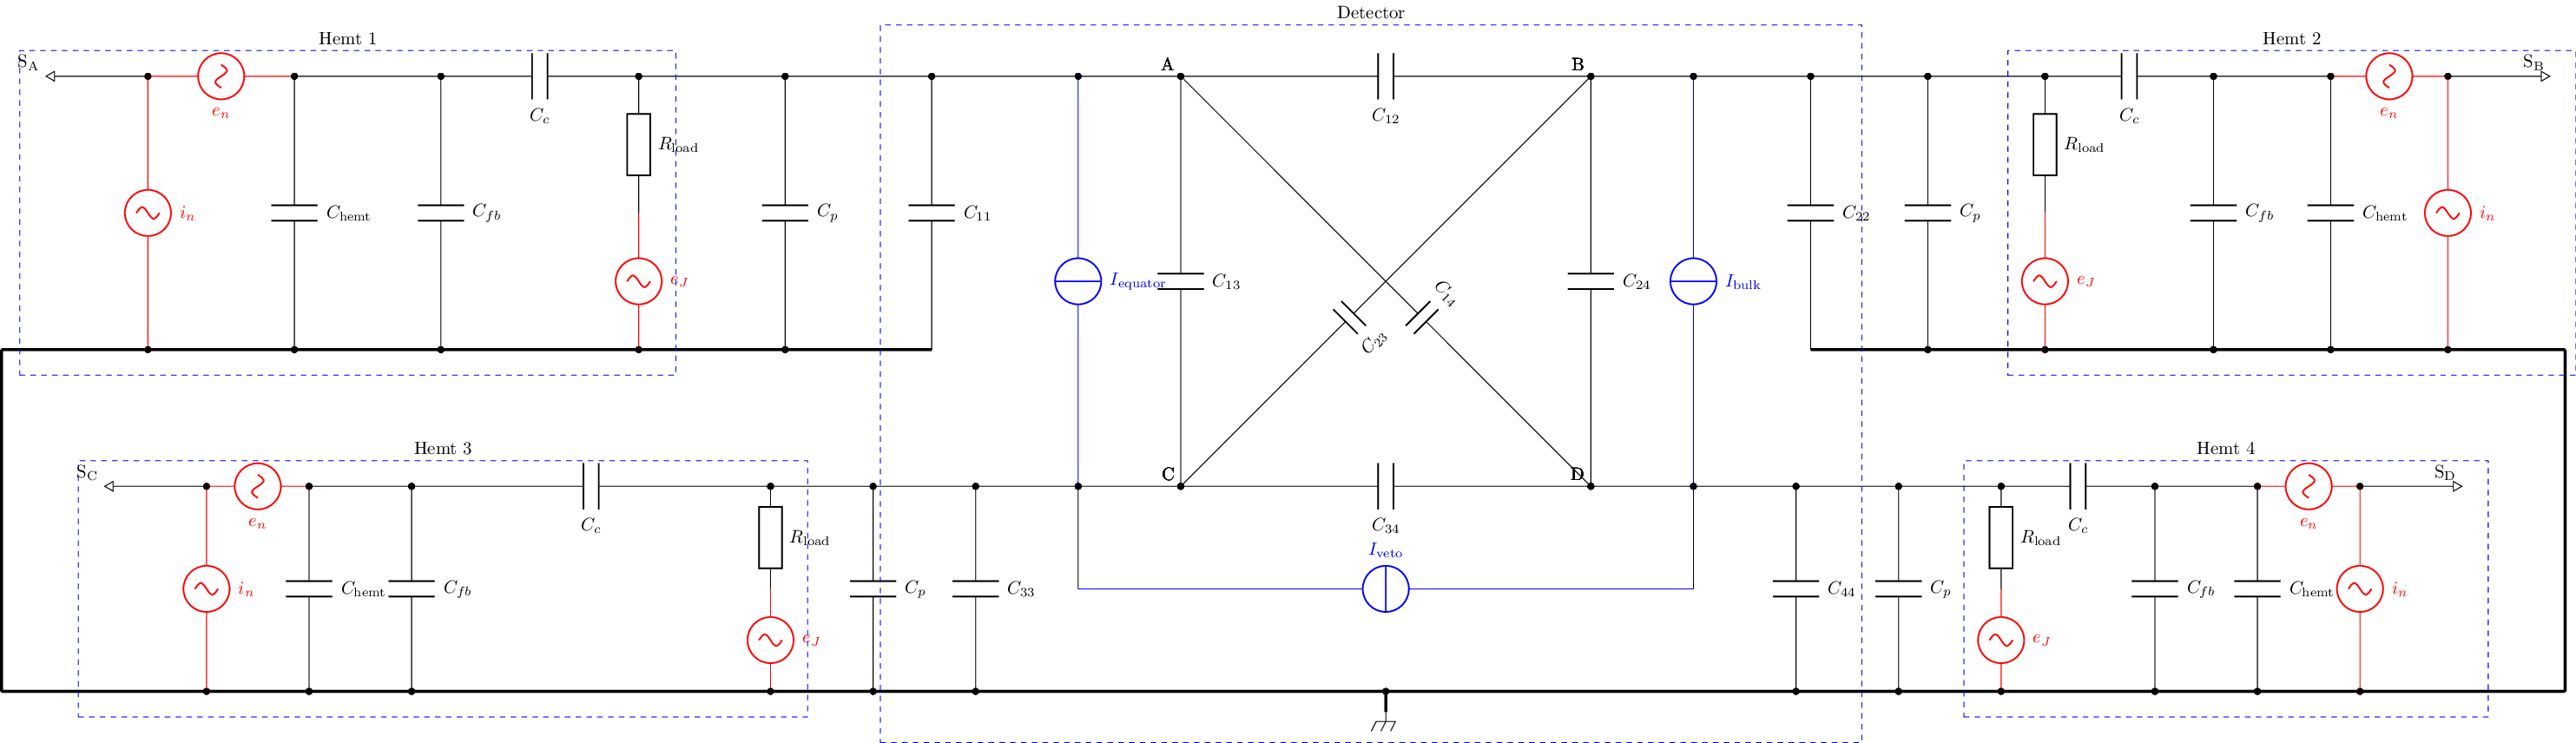
\includegraphics[height=0.25\textheight, width=\linewidth, keepaspectratio]{Figures/Electrodes/scheme_fid38_fat.png}
\caption{Electric scheme of the FID38 with a hemt line for each electrode. The lumped capacitance model is used to represent the capacities of the electrodes. Thus, the scheme uses the term of the mutual capacitance matrix. REDO WITH BETTER FONT SIZE}
\label{fig:scheme-fid38-fat}
\end{figure}

\begin{figure}
\centering
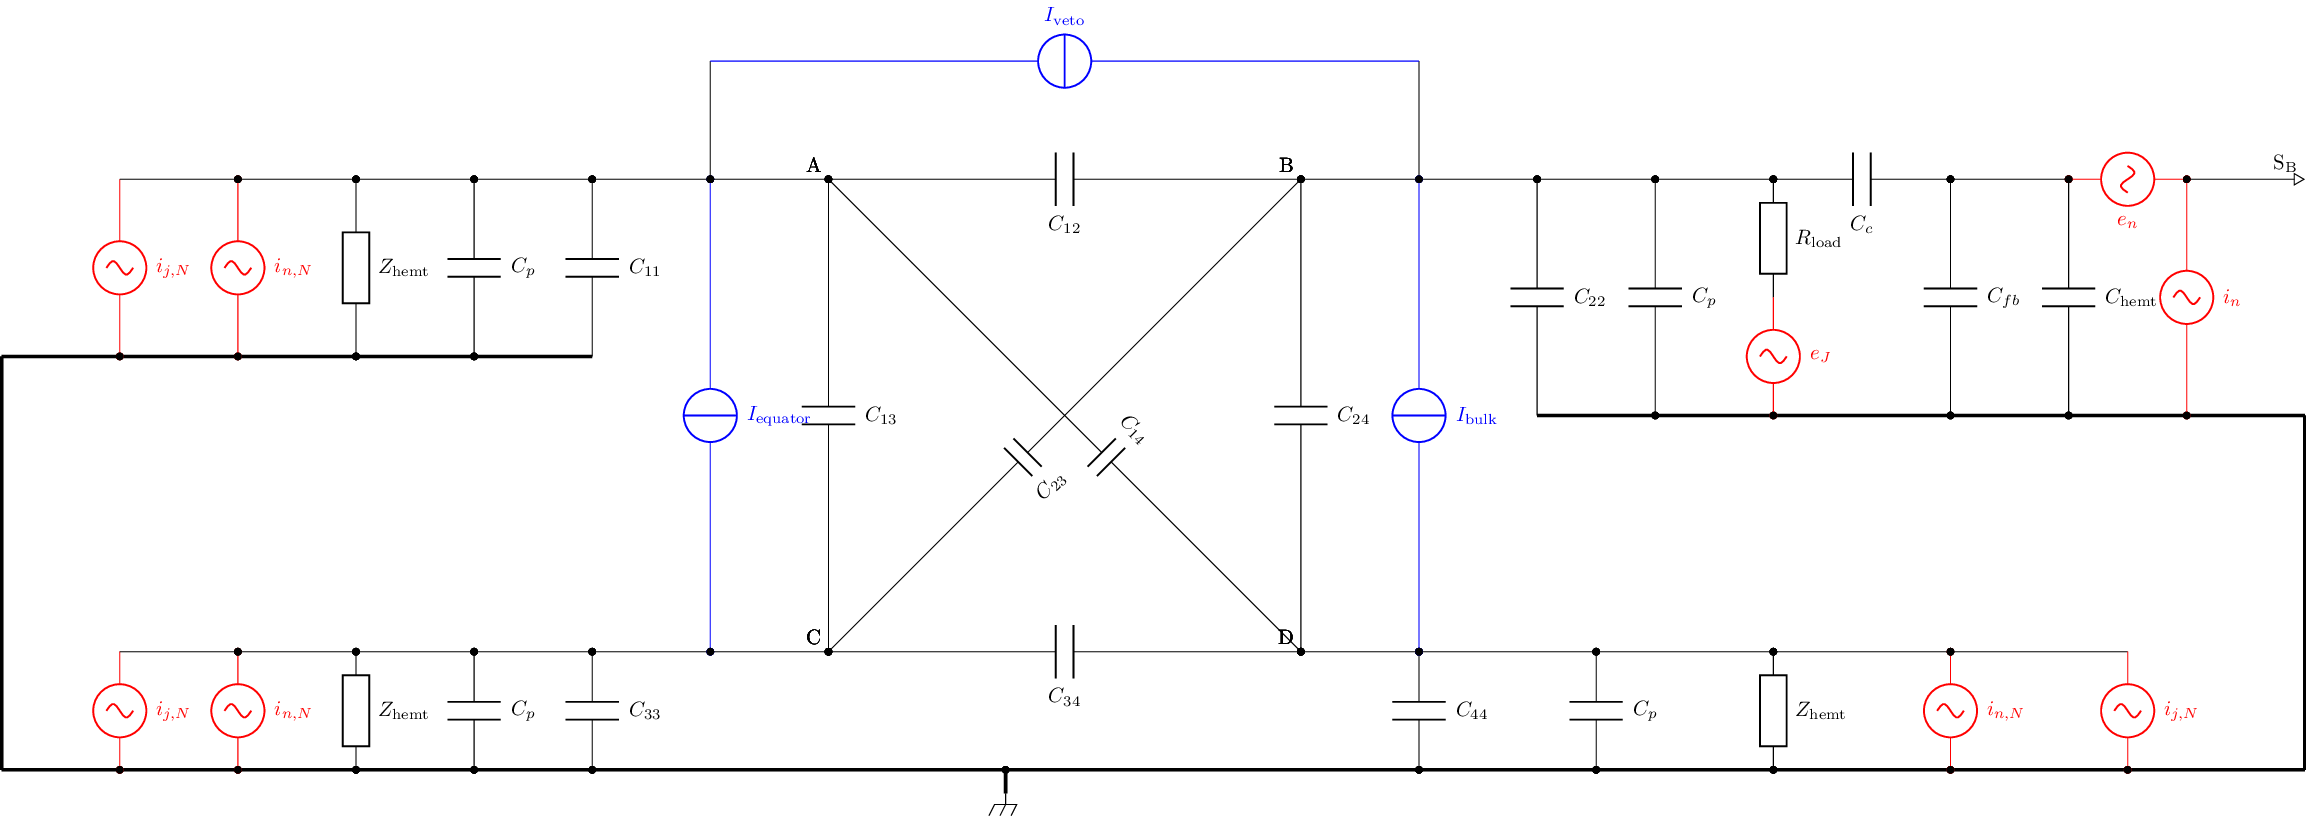
\includegraphics[height=0.25\textheight, width=\linewidth, keepaspectratio]{Figures/Electrodes/scheme_fid38_reduced.png}
\caption{Electric scheme of the Planar38 with a hemt line for each electrode. The lumped capacitance model is used to represent the capacities of the electrodes. Thus, the scheme uses the term of the mutual capacitance matrix. REDO WITH BETTER FONT SIZE}
\label{fig:scheme-fid38-redux}
\end{figure}

\end{landscape}
